%%%%%%%%%%%%%%%%%%%%%%%%%%%%%%%%%%%%%%%%%%%%%%%%%%%%%%%%%%%%%%%%%%%%
%% I, the copyright holder of this work, release this work into the
%% public domain. This applies worldwide. In some countries this may
%% not be legally possible; if so: I grant anyone the right to use
%% this work for any purpose, without any conditions, unless such
%% conditions are required by law.
%%%%%%%%%%%%%%%%%%%%%%%%%%%%%%%%%%%%%%%%%%%%%%%%%%%%%%%%%%%%%%%%%%%%

\documentclass[
  digital, %% This option enables the default options for the
           %% digital version of a document. Replace with `printed`
           %% to enable the default options for the printed version
           %% of a document.
  table,   %% Causes the coloring of tables. Replace with `notable`
           %% to restore plain tables.
  lof,     %% Prints the List of Figures. Replace with `nolof` to
           %% hide the List of Figures.
  lot,     %% Prints the List of Tables. Replace with `nolot` to
           %% hide the List of Tables.
  %% More options are listed in the user guide at
  %% <http://mirrors.ctan.org/macros/latex/contrib/fithesis/guide/mu/sci.pdf>.
  oneside,
]{fithesis3}
%% The following section sets up the locales used in the thesis.
\usepackage[resetfonts]{cmap} %% We need to load the T2A font encoding
\usepackage[T1,T2A]{fontenc}  %% to use the Cyrillic fonts with Russian texts.
\usepackage[
  main=czech,  %% By using `czech` or `english` as the main locale
                %% instead of `slovak`, you can typeset the thesis
                %% in either Czech or English, respectively.
  english, german, russian, czech, slovak %% The additional keys allow
]{babel}        %% foreign texts to be typeset as follows:
%%
%%   \begin{otherlanguage}{german}  ... \end{otherlanguage}
%%   \begin{otherlanguage}{russian} ... \end{otherlanguage}
%%   \begin{otherlanguage}{czech}   ... \end{otherlanguage}
%%   \begin{otherlanguage}{slovak}  ... \end{otherlanguage}
%%
%% For non-Latin scripts, it may be necessary to load additional
%% fonts:
\usepackage{paratype}
\def\textrussian#1{{\usefont{T2A}{PTSerif-TLF}{m}{rm}#1}}
%%
%% The following section sets up the metadata of the thesis.
\thesissetup{
    date            = \the\year/\the\month/\the\day,
    university      = mu,
    faculty         = sci,
    department      = Ústav chemie,
    departmentEn    = Department of Chemistry,
    extra = {
      departmentCs  = Department of Chemistry,
    },
    programme       = Fyzikální chemie,
    programmeEn     = Physical Chemistry,
    extra = {
      programmeCs   = Chemistry,
    },
    field           = Fyzikální chemie,
    fieldEn         = Physical Chemistry,
    extra = {
      fieldCs       = Physical Chemistry,
    },
    type            = mgr,
    author          = Petra Hrozková,
    gender          = f,
    advisor         = doc. Markéta Munzarová Dr. rer. nat. ,
    title           = Studium elektronové struktury fosfosilikátů a jejich silikátových          prekurzorů metodou DFT,
    TeXtitle        = Studium elektronové struktury fosfosilikátů a jejich silikátových          prekurzorů metodou DFT
.
,
    titleEn         = A DFT study of the Electronic Structure of Silicate Precursors for Phosphosilicates
,
    TeXtitleEn      = A DFT study of the Electronic Structure of Silicate Precursors for Phosphosilicates
,
    extra = {
      titleCs       =Studium elektronové struktury fosfosilikátů a jejich silikátových prekurzorů metodou DFT
,
      TeXtitleCs    = Studium elektronové struktury fosfosilikátů a jejich silikátových prekurzorů metodou DFT
,
    },
    keywords        = {kľúčové slovo 1, kľúčové slovo 2, ...},
    TeXkeywords     = {kľúčové slovo 1, kľúčové slovo 2, \ldots},
    keywordsEn      = {keyword1, keyword2, ...},
    TeXkeywordsEn   = {keyword1, keyword2, \ldots},
    extra = {
      keywordsCs    = {klíčové slovo 1, klíčové slovo 2, ...},
      TeXkeywordsCs = {klíčové slovo 1, klíčové slovo 2, \ldots},
    },
    abstract      = {This is the abstract of my thesis, which can

                     span multiple paragraphs.},
    abstractEn    = {This is the English abstract of my thesis, which can

                     span multiple paragraphs.},
    extra = {
      abstractCs   = {This is the Czech abstract of my thesis, which can

                      span multiple paragraphs.},
    },
    thanks        = {These are the acknowledgements for my thesis, which can

                     span multiple paragraphs.},
    bib           = example.bib,
    %% Uncomment the following line (by removing the % symbol at
    %% the beginning) and replace `assignment.pdf` with the
    %% filename of your scanned thesis assignment.
    % assignment    = assignment.pdf,
}
\usepackage{makeidx}      %% The `makeidx` package contains
\makeindex                %% helper commands for index typesetting.
%% These additional packages are used within the document:
\usepackage{paralist} %% Compact list environments
\usepackage{amsmath}  %% Mathematics
\usepackage{amsthm}
\usepackage{amsfonts}
\usepackage{url}      %% Hyperlinks
\usepackage{mhchem}
\usepackage{chemfig}
\usepackage{subfigure}
\usepackage{listings} %% Source code highlighting
\usepackage{braket}
\usepackage{tikz}
\renewcommand{\thesubfigure}{}
%\usepackage{subcaption}
\usepackage{graphicx}
\usetikzlibrary{patterns}
\DeclareRobustCommand{\legendsquare}[1]{%
  \tikz[baseline=(a.south)]{\node[#1, inner sep=.8ex, outer sep=0] (a) {};}%
}
\usepackage{etoolbox}

\newrobustcmd*{\mycircle}[1]{\tikz{\filldraw[draw=#1,fill=#1] (0,0) circle [radius=0.1cm];}}
\newrobustcmd*{\mycircleempty}[1]{\tikz{\draw (0,0) circle [radius=0.1cm];}}
\DeclareUnicodeCharacter{2009}{ }% support older LaTeX versions
\DeclareUnicodeCharacter{2212}{ }% support older LaTeX versions


%\renewcommand{\baselinestretch}{1.2}
%\usepackage{chemmacros}

\lstset{
  basicstyle      = \ttfamily,%
  identifierstyle = \color{black},%
  keywordstyle    = \color{blue},%
  keywordstyle    = {[2]\color{cyan}},%
  keywordstyle    = {[3]\color{olive}},%
  stringstyle     = \color{teal},%
  commentstyle    = \itshape\color{magenta}}
\usepackage{floatrow} %% Putting captions above tables
\floatsetup[table]{capposition=top}
\begin{document}


\chapter{Úvod}


\section{Experimentální motivace}
Cílem této práce je podat vysvětlení některých experimentálních jevů, které byly pozorovány u silikofosfátových polymerů. Studium vysoce porézních silikofosfátů je jedním ze zaměření skupiny anorganické a~materiálové chemie na našem ústavu. Studie prezentované v této práci se zaměřují na na přítomnost hypervalentního, tj. pěti nebo šestikoordinovaného křemíku, v jednotlivých strukturách. Obecný pohled na hypervalency poskytuje Rundleovo a Piementelovo schéma, kde se objevují elektronově-bohaté tří-centerní vazby \cite{405827} \cite{Munzarova2001}.

Amorfní struktura silikofosfátových xerogelů však neumožňuje jejich přímou strukturní charakterizaci. Důležitou součástí práce bylo navržení vhodných strukturních modelů. Modely navržené v této práci byly motivovány rentgenovými strukturami analogických periodických struktur \cite{C3NJ00721A} \cite{C4TA06823H} anebo příbuznými strukturami, které budou dále popsány. Dále byla využita data z NMR spektroskopie, z nichž byly odvozeny informace o výši koordinace křemíku a složení ligandů (fosfátové vs. organické estery)\cite{Styskalik2015thesis}. Druhou součástí práce byl podrobnější pohled na chemickou vazbu ve zvolených modelech silikofosfátových polymerů. Pro analýzu chemické vazby byla použita teorie přirozených orbitalů a Mullikenova populační analýza.

\section{Silikofosfátové polymery}
Nejčastější formou výskytu křemíku v přírodě jsou křemičitany, sloučeniny obsahující křemík tetraedricky koordinovaný čtyřmi atomy kyslíku. Existují však i minerály s vyšší koordinací, např. thaumasit \cite{Edge:a08100}. Vzhledem k vysokému významu křemíku v přírodě jsou křemičitany rozsáhle připravovány a studovány i laboratorně. Oxid křemičitý \ce{SiO2} je po vodě nejvíce studovanou sloučeninou. Díky tomu, že \ce{Si^4+} je velikostně snadno zaměnitelný za \ce{Al^3+} nebo \ce{P^5+}, vznikají pak hlinitokřemičitany, obsahující Si-O-Al (zeolity), nebo fosfokřemičitany, obsahující Si-O-P, tj. silikofosfáty. Obě skupiny sloučenin jsou rozsáhle studovány. Konkrétně silikofosfátové polymery mají zajímavé fyzikální a chemické vlastnosti. Příkladem je Brønstedovská kyselost nebo vysoká protonová vodivost. Několik z možných uplatnění silikofosfátových polymerů mohou být konduktory, elektrolyty, optická vlákna a biokompatibilní materiály.\\

Silikofosfáty i hlinitokřemičitany jsou charakteristické svojí trojrozměrnou  porézní strukturou. Naše pozornost je v této práci soustředěna na silikofosfáty. Předpokládaná struktura připravených silikofosfátů studovaných v předchozích experimentálních pracích je znázorněna na obrázku \ref{si_polymer_cely} \cite{Styskalik2015thesis}. Charakteristickou vlastností struktur silikofosfátů je uspořádání jednotek Si-O-P do cyklů. Ačkoliv nejnovější struktura zahrnuje dvanáctičlenové cykly vzniklé trojnásobným opakování motivu Si-O-P-O (Pinkas et. aln Inorganic Chemistry), struktury s hypervalentním křemíkem obsahující osmičlenné cykly vzniklé dvojnásobným opakováním jednotky Si-O-P-O.
\begin{figure}
\caption{Struktura cyklu 4-členného kruhu z \cite{C4TA06823H};  Legedna: \mycircle{brown} Si, \mycircle{red}~O, \mycircle{orange}~C, \mycircle{yellow} P, \mycircleempty{black}~H.}
 \center 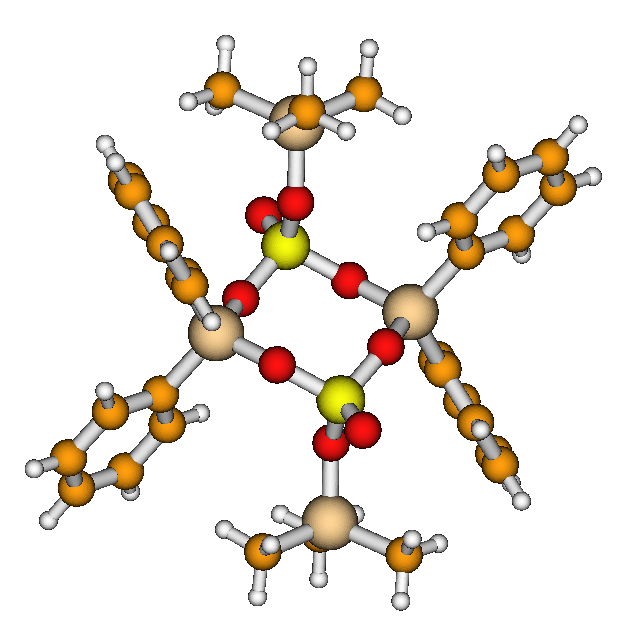
\includegraphics[width=6cm]{rtg_kruh_samostatne.png} \label{rtg_cyklus} \end{figure}
Obrázek \ref{si_polymer_cely} znázorňuje předpokládanou strukturu silikofosfátového xerogelu se třemi druhy křemíkových center (koordinace čtyřmi fosfáty, šesti fosfáty, anebo čtyřmi fosfáty a dvěma organickými estery současně) a osmičlennými cykly Si-O-P.  Konkrétní podoba osmičlenného cyklu byla ověřena metodou RTG \ref{rtg_cyklus}, \cite{C4TA06823H}. Stupeň koordinace křemíku a~současně velikost pórů se ukázala být silně závislá na typu prekurzoru. Pokud byl ve výchozích sloučeninách jeden z fosfátů nahrazen methylovou skupinou přímo vázanou na křemík, ve výsledném xerogelu se nevyskytovaly oktaedricky koordinované křemíky a velikost pórů byla větší. Konkrétní podobu okolí křemíku je ukázáno ve schématu níže \ref{si_polymer_cely}. Podoba koordinačního okolí \ref{koordinacni_okolo} byla získána kombinací NMR dat a IR dat \cite{C4TA06823H} \cite{Styskalik2015thesis}.
\begin{figure}
  \begin{center}
  \begin{tikzpicture}[thick,scale=0.6, every node/.style={scale=0.6}]

  \node at (-4,1) { \chemfig{
                  HO% 2
        -[:330,,2]P% 1
                     (-[:270,,,1]OH% 4
                     )
                     (=[:30]O)% 5
                     %\arrow ([:70]K))
       -[:210,,,2]HO% 3
  }};
    \node at (-2,3)(angle=70){\chemfig{
                   R% 2
            -[:270]Si% 1
                      (
                     <:O% 4
                -[,,,1]P% 7
                      )
                      (
                <[:300]O% 5
            -[:270,,,1]P% 6
                      )
            -[:210]O% 3
        -[:150,,,1]P% 8
    }};
  \draw[-stealth] (-2.65,2.2) -- (-2.2,3.3);
  \node at (4,1.5)  {\small \chemfig{
                  HO% 2
        -[:330,,2]P% 1
                     (
           -[:270,,,1]OH% 4
                     )
                     (
                =[:30]O% 5
                     )
       -[:210,,,2]HO% 3 \schemestop
    }};
  \draw[-stealth] (5.3,2.6) -- (5.8,3.3);
  \draw[-stealth] (7.4,2.4) -- (6.2,3.3);

  \node at (6,3)  {\chemfig{
                   R% 2
            -[:270]Si% 1 \schemestop
                      (
                     <:O% 4
                -[,,,1]P% 7
                      )
                      (
                <[:300]O% 5
            -[:270,,,1]P% 6
                      )
            -[:210]O% 3
        -[:150,,,1]P% 8
    }};
  \node at (9,1.5) { \chemfig{
              O% 2
       =[:330]P% 1
                 (
       -[:270,,,1]OH% 3
                 )
                 (
        -[:60,,,1]OH% 5
                 )
       -[,,,1]OH% 4
    }};
  \end{tikzpicture}
    \end{center}
  \begin{center}
    \begin{tikzpicture}[thick,scale=0.6, every node/.style={scale=0.6}]
      \draw[-stealth] (-2.9,2) -- (-2.2,2.8);
      \draw[-stealth] (5.55,2.45) -- (5.8,2.8);

    \node at (-4.5,1) { \chemfig{
           O% 2
    =[:210]P% 1
              (
        -[:210]O% 4
    -[:240,,,1]Si% 7
              )
              (
        -[:270]O% 5
    -[:330,,,1]Si% 8
              )
    -[:120]O% 3
    -[:150]R% 6
}};
    \node at (-2,3){\chemfig{
               O% 2
     -[:270,,1]Si% 1
                  (
        -[:180,,,1]O% 3
                  )
                  (
      <:[:30,,,1]O% 5
                )
                  (
            -[,,,1]O% 5
                  )
    -[:270,,,1]O% 4
}};
    \node at (4,1.5)  {\chemfig{
           O% 2
    =[:210]P% 1
              (
        -[:210]O% 4
    -[:240,,,1]Si% 7
              )
              (
        -[:270]O% 5
    -[:330,,,1]Si% 8
              )
    -[:120]O% 3
    -[:150]R% 6
}};
    \node at (6,3) {\chemfig{
               O% 2
     -[:270,,1]Si% 1
                  (
        -[:180,,,1]O% 3
                  )
                  (
      <:[:30,,,1]O% 5
                )
                  (
            -[,,,1]O% 5
                  )
    -[:270,,,1]O% 4
}};
  \end{tikzpicture}
  \label{koordinacni_okolo}
  \end{center}
  \caption{Koordinační okolí křemíku v silikofosfátech \cite{C4TA06823H}.}
\end{figure}
Silikofosfátové cykly jsou pak dále organizovány do vyšších struktur mikroporézního (šířka pórů do 2 nm) až mezoporézního (šířka póru 2-50~nm) skeletu. Potvrzená struktura šestikoordinovaného křemíku je uvedena na obrázku \ref{rtg_koordinace_sest} \cite{C3NJ00721A}. Struktura byla získána metodou rentgenové difrakce. Konkrétní metody příprav slikofosfátových sloučenin jsou uvedeny například v práci Aleše Stýskalíka \cite{Styskalik2015thesis}.

\begin{figure}
\caption{Silikofosfátová síť, \cite{Styskalik2015thesis}.}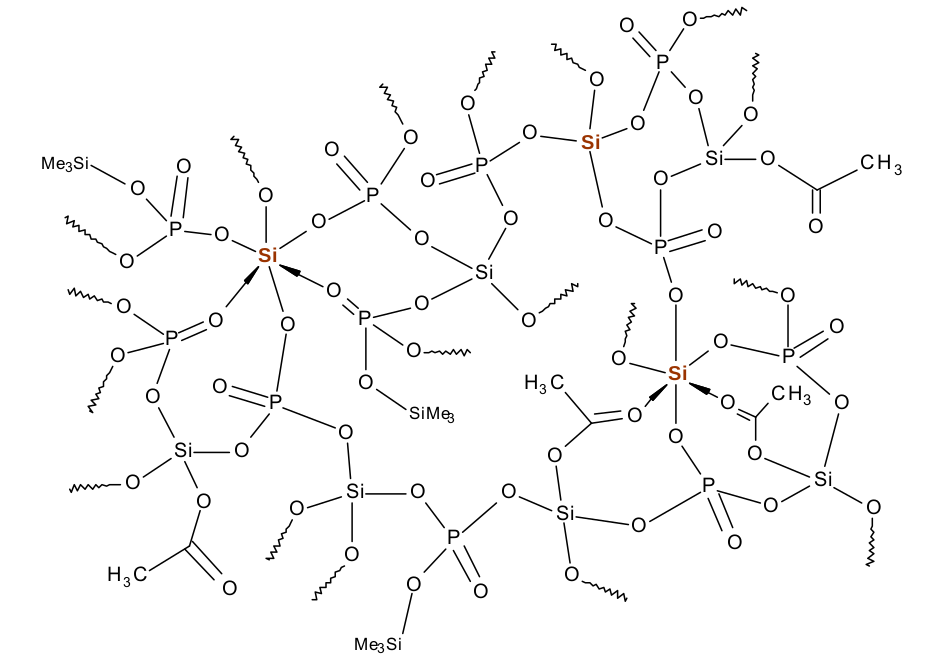
\includegraphics[width=10cm]{si_polymer_cely.png}
\label{si_polymer_cely}\end{figure}

\begin{figure}
\caption{Struktura silikofosfátu získaná z RTG, \cite{C4TA06823H};  Legedna: \mycircle{brown} Si, \mycircle{red}~O, \mycircle{orange}~C, \mycircle{yellow} P, \mycircleempty{black}~H. }
\center 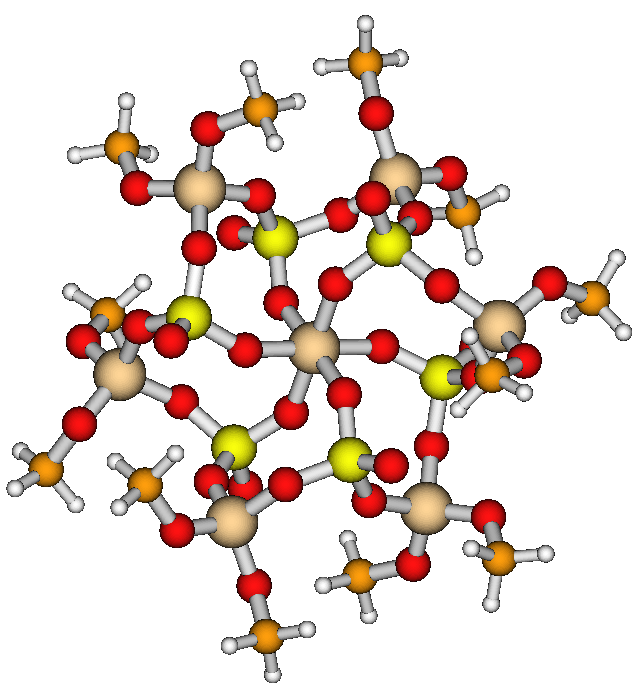
\includegraphics[width=8cm]{struktura_puvodni.png} \label{rtg_koordinace_sest} \end{figure}

\section{Hypervalence $p$-prvků}
První kvantitativní popis chemické vazby zavedl Lewis v roce 1916, kdy vazbu považoval za sdílení elektronového páru mezi dvěma atomy. Cílem párování bylo zaplnění valenčí vrsty a dosažení konfigurace vzácného plynu, tvz. oktetové pravidlo. Pro vodík platí dubletové pravidlo. Pravidlo elektronového oktetu říká, že  prvky $p$ skupiny chtějí mít ve své valenční vrstvě právě osm elektronů. Toho lze docílit vytvořením chemické vazby, excitací nebo ionizací. Spárované elektrony, které se neúčastní vazby, se nazývají volné elektronové páry. Přísná lokalizace elektronů s pomocí vazebných orbitalů v Lewisovské teorii ovšem nesouhlasila s pozorováním pro organické sloučeniny s uhlíkem. Vysvětlení podal L. Pauling pomocí teorie valenčních vazeb a teorie hybridizace \cite{Munzarova1996thesis}.\\

Podle klasické teorie valenční vazby mohou $p$ prvky tvořit čtyři vazby. Z experimentálního pozorování je ale známo, že prvky $p$ bloku tvoří i více vazeb než je číslo jejich atomových orbitalů, obvykle pět nebo šest. Příkladem můhou být sloučeniny xenonu, například \ce{XeF6}.
Sloučeniny, kde se vyskytuje jeden nebo více atomů s více než osmi elektrony (oktet) se nazývají hypervalentní/hyperkoordinované. Konkrétně křemík může vytvářet čtyř, pěti a šestikoordinované sloučeniny a stát se hypervalentní. Pro vysvětlení hypervalence $p$ prvků lze použít teorii hybridizace. Obecně se čtykoordinované sloučeniny vyskytují jako tetraedry, hybridizace $sp^3$. Pětikoordinované sloučeniny tvoří trigonální bipyramidu, hybridizace $sp^3d$. A šestikoordinované sloučeniny tvoří oktaedr, hybridizace $sp^3d^2$ \ref{prehled_koordinaci}.

\begin{figure}
\caption{Přehled koordinaci křemíku.}
\center 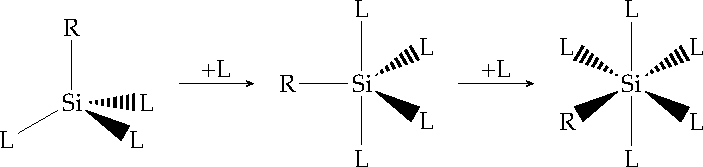
\includegraphics[width=10cm]{drawing.pdf} \label{prehled_koordinaci} \end{figure}

Čtyřkoordinovaný křemík splňuje tetraedrické uspořádání. Při zvýšení koordinace na pět by měla být pozorována trigonální bipyramida, $sp^3d$. Výskyt $d$ orbitalů ve vazbě ale způsobuje nárust energie vazby na více než 200 kcal/mol. Z tohoto důvodu se předpokládá, že $d$ orbitaly se podílejí pouze na polarizaci $p$ orbitalů. Pentavalentní koordinace by měla být realizována jako $3sp^2$ hybridizace doplněna třícenterní, čtyřelektronovou vazbou $3c-4e$ s $p$ orbitalem. V pětikoordinovaných sloučeninách se ale spíše uvažuje hybridizace $sp^2$ a jedna vazba $3c-4e$ s $p$ orbitalem, právě kvůli energii $d$ orbitalů.

Hypervalentní sloučeniny jsou lepší Lewisovské kyseliny díky $d+$ efektu na centralním křemíku. Důvodem je přesun elektronové hustoty na ligandy skrz nevazebné MO a podpora $3c-4e$ vazby. Rozložení elektronové hustoty molekulu stabilizuje a z tohoto důvodu se v hypervalentních sloučeninách vyskytují jako ligandy prvky s vysokou elektronegativitou. Tento jev dobře popisuje tzv. Bentovo pravidlo:"Elektronegativní prvek dáva přednost vazbe s větším p-charakterem" \cite{hypervalentsiliconmacmillangroup2005}. Pro křemík v koordinaci šest lze také předpokládat, že význam $d$ orbitalů nebude významný vzhledem k jejich energii. I zde se do vazby zapojí $3c-4e$ vazby \cite{Wagler2014}.

Další možnost interpretace hypervalence je založena na vysoké iontovosti vazby na křemíku. Obecně iontovost s koordinačním číslem roste.
Navíc chování vazby Si-ligand silně závisí na samotném ligandu a sterickém a elektronovém uspořádání. Hovoříme o Lewisovské kyselosti křemíkové vazby s elektronegativním atomem. Chování křemíku lze rozdělit na iontové, sigma vazebné a donor s interakcí \cite{Wagler2014}.\\


\section{Hypervalence sloučenin křemíku}\label{teorie_hypervalence}
V případě čtyřkoordinovaných sloučenin poskytuje křemík do vazeb všechny své valenční elektorny. Ve vyšším koordinačním stupni už může křemík poskytnou pouze prázdné orbitaly a proto chová se jako Lewisovská kyselina. Obecně mají Lewisovské kyseliny prázdné molekulové orbitaly, které leží dostatečně blízko obsazeným molekulovým orbitalů (MO)\footnote{MO - \textit{Molecular orbital}} konjugované báze.
\begin{figure}
\begin{center}
\subfigure[]{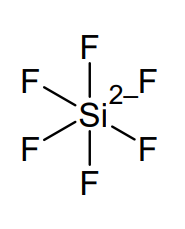
\includegraphics[width=2cm]{si_f6.png}\label{si_f6}}
\subfigure[]{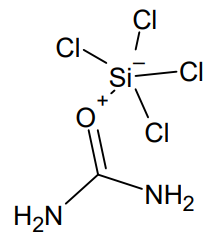
\includegraphics[width=3cm]{si_cl_o.png}\label{si_cl_o}}
\subfigure[]{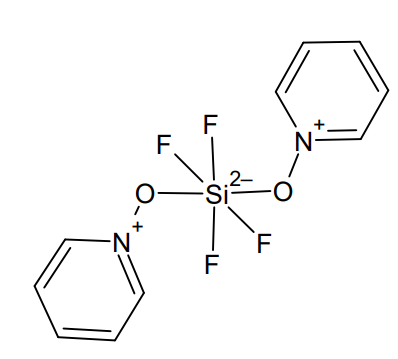
\includegraphics[width=5cm]{si_o_f.png}\label{si_o_f}}
\subfigure[]{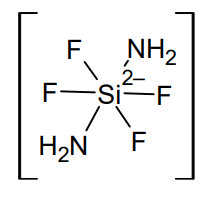
\includegraphics[width=3cm]{si_f_n.png}\label{si_f_n}}
\subfigure[]{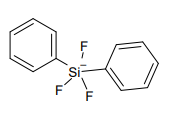
\includegraphics[width=5cm]{si_with_fluor_carbons.png} \label{si_with_fluor_carbons}}
\subfigure[]{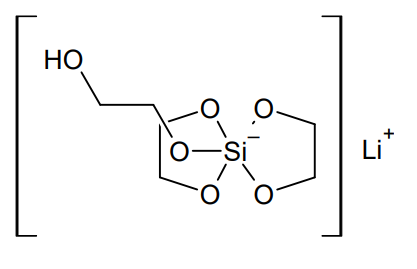
\includegraphics[width=5cm]{si_only_o.png} \label{si_only_o}}
\subfigure[]{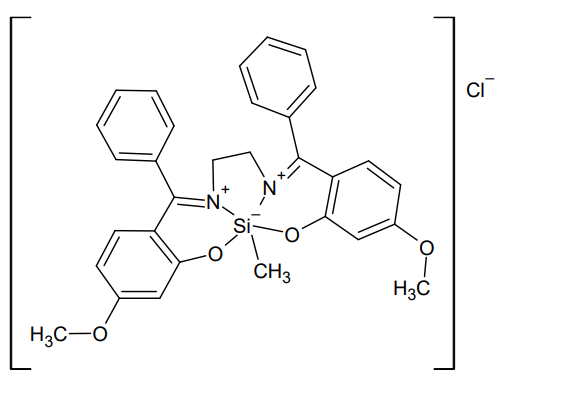
\includegraphics[width=5cm]{si_n_o_c.png}\label{si_n_o_c}}
\subfigure[]{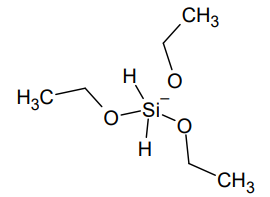
\includegraphics[width=5cm]{si_fluor_vodik_kyslik.png} \label{si_fluor_vodik_kyslik}}
\subfigure[]{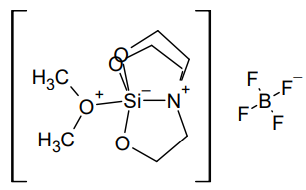
\includegraphics[width=5cm]{si_o_n.png} \label{si_o_n}}
\subfigure[]{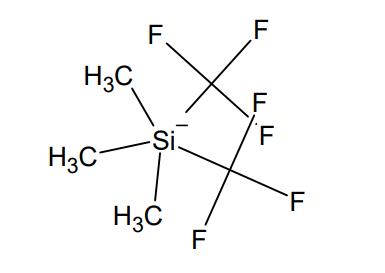
\includegraphics[width=5cm]{si_only_c.png} \label{si_only_c}}
\label{shrnuti_struktury_kremik}
\end{center}
\end{figure}
Z experimentu je známo, že \ce{SiO4} je dostatečnou Lewisovskou kyselinou, aby křemík mohl přímo reagovat s Lewivoskou bazí. Pokud je jeden z kyslíku ve struktuře nahrazen uhlíkem, schopnost navyšovat koordinaci je ztracena. Stejný jev pozoroval Aleš Sýskalík a spol. \cite{Styskalik2015thesis} a to vedlo k hypotézi o snížení Lewisovské kyselosti křemíku při tvorbě přímé vazby Si-C. Naopak pětikoordinovaný křemík je lepší Lewisovskou kyselinou než čtyřkoordinovaný křemík a hypervalency podporuje. Atomy jako uhlík, dusík, kyslík, fluor nebo chlor podporují navyšování koordinace křemíku \cite{Wagler2014}.\\

Existující, experimentálně připravené hypervalentní sloučeniny s křemíkem lze rozdělit podle jednotlivých ligandů a jejich poloze v periodické tabulce. Křemík je schopen tvořit hypervalentní sloučeniny s fluorem, příkladem může být struktura  \ce{(SiF6)^{2-}} \ref{si_f6} \cite{memoriesphysiquelussac}. Tato struktura byla připravena v 19. století a považuje se za první připravenou sloučeninu křemíku v koordinaci šest. Pokud budeme postupovat ve skupine halogenů dolů, dalším ligandem by měl být logicky chlor. Sloučenina \ce{SiCl6^{2-}} ale není známá, naopak \ce{GeCl6^{2-}} ano. Schopnost atomu tvořit hypervalentní sloučeniny roste ve skupině dolů. Germanium má tedy vysokou schopnost tvořit hypervalentní sloučeniny. Oproti tomu křemík potřebuje ligand s výrazně vyšší elektronegativitou. Hypervalentní sloučeniny s chlorem byly proto připraveny až později, například \ref{si_cl_o} \cite{LAZAREV199716}.

Ve sloučeninách s křemíkem může být fluor nahrazen dalšími $p$ prvky, například kyslíkem \ref{si_o_f} \cite{C0DT01115K} nebo kyslíkem a vodíkem \ref{si_fluor_vodik_kyslik} \cite{BOYER19812165}.
Jako ligand společně s fluorem může být použit i dusík \ref{si_f_n} \cite{C0DT01115K} nebo uhlík \ref{si_with_fluor_carbons} \cite{kremikfluorcarbon}. Schopnost křemíku navyšovat koordinaci existuje i ve sloučeninách s kyslíkem \ref{si_only_o} \cite{flyn1969}. Strukutra \ce{SiO6} se vyskytuje také v přírodě v minerálu thaumasitu \cite{Edge:a08100}. Kyslík může být nahrazen dusíkem  \ref{si_o_n} \cite{Wagler2014} nebo uhlíkem a dusíkem  \ref{si_n_o_c} \cite{Wagler2014}. Je zajímavostí, že existují i sloučeniny pouze s vazbou křemík-uhlík \ref{si_only_c} \cite{A901953G} \cite{Wagler2014}.

\section{Formulace teoretického problému}
Postupně jsme hlavní otázku, řešenou v této práci, zformulovali do následující podoby: Jaká je souvislost mezi kombinací ligandů na čtyřkoordinovaném křemíku a Lewisovskou kyselostí těchto čtyřkoordinovaných sloučenin, vedoucí ke sklonu křemíku zvýšit svoji koordinaci na pět nebo šest ligandů.
Z tohoto důvod jsme se rozhodli porovnávat Lewisovskou kyselost, abychom určili stabilitu jednotlivých částí silikofosfátů. Navíc jsme se snažili najít parametr, který by umožnil určit velikost póru v závislosti na okolí křemíku. Pro tuto práci jsem zvolila tři úrovně zkoumání silikofosfátů, rozdělené podle velikosti modelů. Velké modely sloužily jako odhad skutečné struktury silikofosfátů, včetně jednotlivých pórů. Středně velké modely byly stále dost komplexní, ale již umožňovaly podrobnější pohled na chemickou vazbu Si-C. Malé modely byly snadné pro porozumění.

Jako prostředek ke zkoumání silikofosfátů jsem zvolila molekulové orbitaly, které poskytují široké spektrum informací o molekule, vazbách, struktuře, kyselosti, \dots.  Analýza byla provedena s pomocí teorie funkcionální hustoty (DFT)\footnote{DFT - \textit{Density Functional Theory}, česky Teorie funkcionálu hustoty}, která se řadí mezi kvantově-chemické metody. Pro porovnání byla stejná analýza udělána s pomocí teorie přirozených molekulových orbitalů (NBO)\footnote{NBO - \textit{Natural Bond Orbitals}, česky Přirozené Molekulové orbitaly}. Výhoda přístupu NBO je snadnější převod číselných výsledků do tradičního chemického významu. Pro určení Lewisovské kyselosti bylo stěžejní určení procenta $s$ a $p$ orbitalů křemíku v antivazebných orbitalech.  V NBO analýze jsme určovali procento vazebných orbitalů (BD) \footnote{BD - \textit{Bond Orbital}} a protivazebných (BD*) orbitalů křemíku a ligandu. V MPA\footnote{MPA - \textit{Mulliken's Population Analysis}, česky Mullikenova populační analýza} analýze jsme určovali procento $s$~a~$p$ orbitalů křemíku a okolních ligandech.
\newpage

\chapter{Metody kvantové chemie}
Chování elektronů v molekulách však nelze popsat rovnicemi ani jazykem klasické mechaniky. Elektrony totiž vykazují typické kvantově-mechanické chování, projevující se diskrétním spektrem energií, vlnovým chováním ve smyslu difrakce nebo např. fotoelektrickým jevem. Nelze je proto charakterizovat jejich jednotlivými polohami a hybnostmí, jediný přijatelný popis lze udělat pomocí tzv. vlnové funkce.
\section{Kvantově-mechanický popis elektronové struktury}
Současné chápání struktury, reaktivity a spektroskopického chování látek je založeno na detailní znalosti rozložení elektronů a jejich energiích v atomech a molekulách. Vlnová funkce se zpravidla označuje řeckým písmene $\Psi$ a je řešením Schrödingerovy vlnové rovnice \ref{schr_rce}. Levá strana Schrödingerovy rovnice vyjadřuje působení tzv. Hamiltoniánu ($\widehat{H}$) neboli operátoru energie na vlnovou funkci $\Psi$. Pravá strana Schrödingerovy rovnice vyjadřuje fakt, že lze nalézt takové vlnové funkce $\Psi$, které se působením operátoru $\widehat{H}$ pouze vynásobí konstantou $E$, která má význam energie. Řešením Schrödingerovy rovnice jsou tedy jednak možné hodnoty energie elektronů sytemu a jednak samotná vlnová funkce $\Psi$, která v sobě dle tzv. Bornovy interpretace obsahuje informaci o rozložení pravděpodobnosti vsýktytu elektronů v prostoru.
\begin{equation}
\widehat{H} \Psi = E \Psi,
\label{schr_rce}
\end{equation}
Analytická řešení Schrödingerovy rovnice jsou dostupná pouze pro velmi malý okruh jednoduchých modelových Hamiltoniánů, jejiž nejdůležitějšími reprezentaty jsou kvantově-chemický oscilátor, částice v jámě, atom vodíku a kation \ce{H2^{+}}. Dokonce ani pro atomu helia, který obsahuje pouze o jeden elektron více než atom vodíku, není dostupné plně analytické řešení Schrödingerovy rovnice.
Z tohoto důvodu je ve fyzikálních i chemických aplikacích nutno použít zjednodušení. Základní aproximací, kterou je třeba aplikovat pro všechny molekuly (včetně zmiňovaného iontu \ce{H2^{+}}, pro nejž lze vlnovou funkci elektronu vyjádřit analyticky) je tzv. Born-Oppenheimerova aproximace (B-O) \ref{B_O_approximace}.
Její podstatou je oddělení pohybu elektronů od pohybu jader a lze ji dobře vysvětlit na základě termodynamické analogie vratného děje. Je-li například expanze plynu proti vnějšímu tlaku prováděna vratně, pohybuje se píst ve válci tak pomalu, že plyn je stále v rovnováze s okolím. Jeho tlak pak závisí pouze na pozici pístu. Podobně se jádra pohybují vzhledem k elektronům tak pomalu, že elektrony zaujmou pro každé rozmístění jader okamžitě nejvýhodnější rozložení. Proto můžeme energii elektronů považovat za závislou pouze na polohách jader. V rámci B-O aproximace lze tedy vlnovou funkci zapsat ve tvaru rovnice \ref{B_O_approximace}.
\begin{equation}
  \Psi_{r_i,R_{\alpha}} = \Psi_{electronic}(r_i,R_{\alpha}) \cdot \Psi_{nuclear}(R_{\alpha}),
  \label{B_O_approximace}
\end{equation}
$R_{\alpha}$ jsou souřadnice jader, $\Psi_{electronic}(r_i,R_{\alpha})$ je elektornová vlnová funkce, zavisející explicitně na polohách elektronů a parametricky na polohách jader. $\Psi_N(R_{\alpha})$ je jaderná vlnová funkce závislá pouze na polohách jader. $ \Psi_{nuclear}(r_i, R_{\alpha}) $ je celková vlnová funkce \cite{lechamolecularmodeling}.
Vlnová funkce elektronů je řešením Schrödingerovy rovnice, jež v operátoru energie zahrnuje pro každý elektron jeho kinetickou energii, přitahování elektronu jádry a jeho odpuzování se všemi ostatními elektrony. Poslední jmenovaný člen řídí pohyb každého elektronu a je závislý na pohybu všech ostatních elektronů. V důsledků toho není elektronová Schrödingerova rovnice analyticky řešitelná. \\

Druhou základní aproximací kvantové chemie je přístup, v němž se okamžitá repulze jednoho elektronu s druhým nahrazuje repulzí prvního elektornu v časově rozmazanou distribucí druhého elektronu. Cílem je pak nalézt takové vlnové funkce obou (a všech dalších) jednotlivých elektronů, aby pro jeden elektron byla vlnová funkce tzv. orbital-optimální z hlediska minimalizace celkové energie. Tady například vlnová funkce pro elektron jedna musí být optimální mj. vzhledem k repulzím s elektronem dvě a obráceně, vlnová funkce pro elektro dva musí být optimální mj. vzhledem k repulzím s elektronem jedna. Celková vlnová funkce daného počtu elektronů, která se vyjadřuje jako tzv. Slaterův determinat z obsazených orbitalů, musí být z tohoto hlediska konzistentní sama se sebou, a proto se výše pospaná metoda nazývá Hartee-Fockova metoda selkonzistentního pole (HF-SCF) \footnote{HF-SCF - \textit{Hartree-Fock Method Self-Consistent Field}}. Vlnovou funkci lze zapsat jako Slaterův determinant (SD), který zaručuje antisymetrii vlnové funkce vůči výměně polohových a spinových souřadnic \ref{Slateruv_determinant}.
\begin{equation}
\psi =  \frac{1}{\sqrt{N!}}\begin{vmatrix}
\psi_1(1)\alpha(1) & \psi_1(1) \beta (1)  & \dots & \psi_{n/2}(1)\beta(1) \\
\psi_1(2)\alpha(2) & \psi_1(2) \beta (2) & \dots & \psi_{n/2}(2)\beta(2) \\
\vdots             & \vdots                           & \ddots & \vdots \\
\psi_1(n)\alpha(n) & \psi_1(n) \beta (n) & \dots & \psi_{n/2}(n)\beta(n)
\end{vmatrix}
\label{Slateruv_determinant}
\end{equation}
$\psi_i$ jsou prostorové části jednotlivých orbitalů, 1,2,\dots n jsou jednotlivé elektrony $i$, $\alpha(i)$ resp. $\beta(i)$ jsou spinové funkce těchto elektronů a $\frac{1}{\sqrt{N!}}$ je normovací konstanta.

Výsledná vlnová funkce se hledá následujícím způsobem: Na počátku výpočtu je zvolena určitá sada orbitalů, které jsou postupně jednotlivě optimalizovány v poli elektronové hustoty zbylých orbitalů. Tím získáme novou sadu orbitalů, která se liší od původní sady orbitalů. Celý postup je opakován až do okmažiku, kdy mezi předchozí a následující sadou orbitalů rozdíly v energiích a elektronové hustotě klesnou pod předem zvolenou, dostatečně nízkou mez. Protože jsou výsledné energie vlastními funkcemi tzv. Fockova operátoru, který patří mezi tzv. Hermitovské operátory, jsou vypočítané orbitaly $\Psi_i$ a $\Psi_j$ příslušející různým vlastním hodnotám energie $\varepsilon_i $ a $\varepsilon_j$ orthogonální, tj. platí rovnice \ref{ortogonal}. Navíc lze zajistit, aby byly orthogonální každé dvě vlnové funkce příslušející stejné vlastní hodnotě energie $\varepsilon_i$, a také, aby každá vlnová funkce $\varphi_i$ tj. \ref{ortonormal} byla normovaná.
 \begin{equation}
S_{ij} = \int \psi_i * \psi_j dx dy dz = 0,
 \label{ortogonal}
 \end{equation}
 \begin{equation}
   S_{ii} = \int \psi_i * \psi_i dx dy dz = 1,
   \label{ortonormal}
 \end{equation}
Nejnižší energie se hledá pomocí selfkonzistentní metody (viz. výše). Nevýhoda HF-SCF přístupu je fakt, že neuvažuje korelaci elektronového pohybu, tj. fakt, že vybraný elektron nevnímá ostatní elektrony v jejich časově zprůměrovaném rozložení, nýbrž že vnímá okamžité polohy ostatních elektronů a přizpůsobuje jim svoji polohu.\\

Korelační energii lze vyjádřit jako rozdíl mezi přesnou nerelativistickou energii a HF limitou tzv. Hartree-Fockovou limitou, což je energie Slaterova determinant, vyjádřeného v limitě nekonenčné báze. Ačkoliv korelační energie představuje méně než 1\% celkové tzv. energie elektronů, nemůže být zanedbána, pokud požadujeme chemickou přesnost tj. $1-2$ kcal/mol.

Korelační energii lze do výpočtu zahrnout tak, že výsledná vlnová funkce obsahuje mimo Slaterův determinant pro základnní stav také příspěvky Slaterových determinantů pro excitované stavy. Hovoříme pak o Post-Hartree-Fockových metodách. Mísením excitovaných determinantů lze započítat třemi základními způsoby. Předně jde o tzv. metodu konfigurační interakce (CI)\footnote{CI - \textit{Configuration Interaction}}, v níž jsou příspěvky excitací optimalizovány pomocí variační metody. Jiným možným způsobem započtení excitovaných determinantů je poruchová teorie zavedená M{\o}llerem a Plessetem. Poslední (a v reálné praxi nejpřesnější) metodou zahrnutí korelace pohybu elektronů prostřednictvím jejich excitaci do protivazebných MO je tzv. metoda spřažených klastrů. Její výhoda oproti CI je její správné škálování s velikostí systému díky tomu, že jednotlivými excitacemi zahrnuje i jejich superpozice.

 %#TODO poznámky k teoriím
\section{Teorie funkcionálu hustoty}
Systémy studované v této práci mají za cíl modelovat trojrozměrnou silikofosfátovou síť. Skládají se tedy ze silikátových a fosfátových jednotek, z nichž na každou jednotku připadá cca. 50 elektronů. Je proto velice důležité zvolit metodu, která bude spojovat vysokou přesnost s vysokou výpočetní efektivností. Současně je našim cílem porozumění sklonu křemíku k hypervalenci, což indikuje pokud možno fyzikálně průzračný jednoelektronový model. Všechny tyto požadavky splňuje Kohn-Shamova formulace metody funkcionálu hustoty\footnote{Z matematické analýzy je funkcionál operátor zobrazení z množiny funkcí do množiny obecně komplexních čísel.}\cite{bickelhaupt2007kohn}.

Základní myšlenka teorie funkcionálu hustoty pohlíží na systém elektronů a jader ze zcela jiného úhlu než tradiční \textit{ab inito} metody kvantové chemie, zahrnující metodu HF-SCF a její nadstavby. Posledně zmíněné metody zahajují popis molekuly od znalosti tzv. externího potenciálu (nejčastěji daného polohami a náboji jader) a pokračují přes konstrukci Hamiltoniánu, nalezení energií a vlnových funkcí až k výpočtu výsledné elektronové hustoty.

Základní teorémy metody funkcionálu hustoty (1. a 2. Hohensberg-Kohnův teorém) ukazují, že lze postupovat i opačně. Výsledná elektronová hustota zpětně jednoznačně určuje externí potenciál, a tedy i vlnovou funkci a všechny z ní odvozené měřitelné vlasnosti. Protože je elektronová hustota funkcí pouze tří souřadnic v prostoru (a nevztahuje se narozdíl od vlnové funkce k jednotlivým elektronům), lze metody funkcionálu hustoty využít k výpočtům, které jsou do výpočetní náročnosti srovnatelné s metodou HF-SCF, ale co do přenosti popisu metodu HF-SCF dalece převyšují \cite{jensen2007introduction}.\\

Moderní DFT\footnote{DFT - \textit{Density Functional Theory}} metody se začaly objevovat po roce 1964 jako výsledek Hohensberg-Kohnova teorému. Aplikace v kvantově-chemických výpočtech se datují od 90. let. První Hohenberg-Kohn teorém (H-K) mluví o základním stavu. "Vnější potenciál  $V_ext$ je až na konstantu jednoznačným funkcionálem $\varrho(\vec{r})$, protože $V_ext$ určuje $\widehat{H}$, je úplný popis mnohačásticového základního stavu jednoznačným funkconálem $\varrho(\vec{r})$."\cite{PhysRev.136.B864} První H-K teorém můžeme schématicky vyjádřit takto:
\begin{equation}
\varrho_0 \Rightarrow \{N, Z_A, R_A\} \Rightarrow \widehat{H} \Rightarrow \Psi_0 \Rightarrow E_0,
 \end{equation}
 Všechny vlastnosti základního stavu mnohaelektronového systému jsou tedy jednoznačně určeny elektronovou hustotou. Návodem pro získání elektronové hustota je druhý teorém. Obsahem druhého H-K teorému je variační princip, který lze v našem kontextu vyjádřit následovně.
\begin{equation}
E_0 < E [\tilde{\varrho}] = T[\tilde{\varrho}] + E_{Ne}[\tilde{\varrho}] + E_{ee}[\tilde{\varrho}],
\end{equation}
Kde $\tilde{\varrho}(\vec{r})$ je zkušební hustota, splňující vazbené podmínky. Pro výpočetní chemii mají větší význam Kohn-Shamovy (K-S) orbitaly, které byly výsledkem geniální myšlenky o rozdělení funkcionálu. Obecně je největší problém vyjádřit kinetickou energii elektornů. Ta se rozpadla na dvě části. Exaktní a korekční část  \cite{jensen2007introduction}\cite{koch2000chemist}.
\begin{equation}
E(\varrho(\vec{r})) = T_s[\varrho(\vec{r})] + J[\varrho(\vec{r})] + \int V_{EX}(\vec{r})\varrho(\vec{r})d\vec{r} + E_{XC}[\varrho(\vec{r})],
\end{equation}
 \begin{equation}
 T_s = -\frac{1}{2} \sum_{i=1}^{N}  \bra{\psi_i}{\nabla^{2}}\ket{\psi_i},
 \label{kineticka_energie_jednoelektronova}
 \end{equation}
 Kinetická energie $T_s$ ale není přesným vyjádřením kinetické energie. Chybějící část je zajištěna $E_{EX}[\varrho(\vec{r})]$, výměnná-korelační energie. $J[\varrho(\vec{r})]$ je přesná Coulombovská repulze. $\int V_{EX}(\vec{r})\varrho(\vec{r})d\vec{r}$ je přesná energie atrakce elektronů jádry \cite{parr1994density}.
%#TODO dodělat úvod k DFT
\subsection{DFT metody v praxi}
Největším problémem při aplikaci DFT je nalezení vhodného výměně-korelačního potenciálu. V principu přesný K-S přístup neříká nic o tom, jak výměně-korelační potenciál nalézt. Existují dva způsoby hledání tohoto parametru. První hledá vhodný $E_{EX}$ z teorie, jedná se o čistý $ab inito$ přístup. Druhý přístup hledá parametry pro $E_{EX}$, které lze určit z experimentálních dat.

První přístup se ozačuje jako aproximace lokální hustoty(LDA)\footnote{LDA = \textit{The Local Density Approximations}} a vychází z modelu homogenního elektronového plynu. Jedná se o hypotetický stav, kde se elektorny pohybují na kladném pozadí a celkový náboj je neutrální. Celý prostor se rozdělí na jednotky objemu a elektronová hustota se počítá vždy ve středu tohoto objektu. Celkovou energii najdeme jako součet přes všechny objemy. Tento model je vhodný pro jednoduché kovy, napříkald sodík. S jeho pomocí lze popsat valenční elektorny v kovech. Význam LDA modelu je, že je to jediný systém, pro který známe přesně $E_{EX}$ část. Vylepšením LDA modelu je oddělení práce s elektronovou hustotou elektronů se spinem $\alpha$ a $\beta$, označováno jako LSDA\footnote{LSDA - \textit{Local Spin Denstiy Approximation}}. Nevýhodou je, že obě metody nelze dobře použít pro nehomogenní elektrostatické pole molekul a pro chemické reakce.

 Druhým přístupem je metoda gradientu hustoty (GGA)\footnote{GGA -\textit{Generalized Gradient Approximations}}. S pomocí Taylorova rozvoje lze z lokálních hodnoty elektronové hustoty v daném objemu získat gradient hustoty $\nabla \varrho(\vec{r})$, výměnný-korelační funkcionál má obecný tvar \ref{gga}.
\begin{equation}
  E_{XC}^{GGA} = \int \varrho(\vec{r})f(\varrho, \nabla_{\varrho})d\vec{r}
  \label{gga}
\end{equation}
 Nejvýznamějším funkcionál je Beckeho výměnný funkcionál (B88) s jedním parametrem. Dalším známým GGA funkcionálem je LYP \cite{lyp} nebo BLYP \cite{blyp}. Práce v oblasti GGA funkcionálů vedly k rozšíření DFT i v kvantové chemii.

 Třetí významnou a v kvantové chemii nejpoužívanější skupinou funkcionálů jsou hybridní funkcionály. Hybridní funkcionály jsou kombinací čistého DFT přístupu a přesné HF výměny. Část výměně-korelační energie vypočítáme s K-S orbitalů a druhou část s předchozích funkcionálů.
\begin{equation}
  E_{XC} = E_{X}^{exact} + E_C^{K-S}
\end{equation}
Nejznámějším funkcionálem je B3LYP \cite{b3lyp}, navržen v roce 1994.
\begin{equation}
  E_{XC}^{B3LYP} = (1-a)E_{X}^{LSD} + a \cdot E_{XC}^{\lambda = 0} + b \cdot E_{X}^{B88} + c \cdot E_{C}^{LYP} + (1-c)E_{C}^{LSD}.
\end{equation}
$\lambda$ je .Funkcionál B3LYP je dodnes považován za univerzální a nejpoužívanější funkcionál. Nachází využití v mnoha chemických aplikacích \cite{koch2000chemist}.

 \subsection{Spektroskopické vlastnosti atomů a molekul}
 Chemický posun v NMR je jednou z nejdůležitějších magnetických vlastností chemických látek. Kvantově-mechanické metody popsané výše lze využít k výpočtu dovolených hladin energie a jim odpovídajících vlnových funkcí. Z vlnových funkcí ale dle postulátů kvantové mechaniky vyplývají všechny pozorovatelné vlastnosti systému, tedy například odpověď na vnější magnetické pole. Externí magnetické pole $\vec{B}_0$ totiž interaguje s orbitalními momenty hybnosti jednotlivých elektronů. Tím se vytváří dostatečné magnetické pole $\delta \vec{B}$ působící na jádro. Přídavné pole $\delta \vec{B}$ odpovídá vnějšímu poli $\vec{B}$ vztahem:
\begin{equation}
  \delta \vec{B} = - \sigma \vec{B}_0,
\end{equation}
kde $\sigma$ je tzv. stínící konstanta (většinou kladá, někdy však záporná) \cite{atkins2010atkins}.
%#TODO atkins, definice chemického posunu, strana 496

 $B_0$, které je reprezentováno vektorovým potenciálem tohoto pole. V~ideálním případě by neměla mít volba počátku tohoto pole vliv na výsledek. Jedním z~důsledků aproximace v~kvantové chemii je fakt, že volba počátku výrazně ovlivňuje výsledné chemické stínění. Problém se nazývá \uv{Gauge origin problem}. Metoda GIAO \cite{giao} (Gauge  Including Atomic Orbitals) řeší problém způsobem, že zahrnuje počátek vektorového potenciálu do atomových orbitalů nebo do lokalizovaných molekulových orbitalů (IGLO)\footnote{IGLO - \textit{giao}}. Vhodnou bazí pro tyto výpočty je IGLO$-$III \cite{Standara2006thesis} (Individual Gauge for Localized Orbitals) \cite{g09}.

\section{Báze v kvantově chmemických výpočtech}
Základním přístupem pro hledání molekulových orbitalů je metoda MO-LCAO \footnote{MO-LCAO - \textit{Molecular Orbital – Linear Combination of Atomic Orbitals}}, která je založena na postulátu o úplnosti systému vlastních funkcí. Podle postulátu QM o úplných vlastních hodnotách uplných Hermitovských operátorů lze každý molekulový orbital sestrojit jako lineární kombinaci atomových orbitalů, tzv. LCAO\footnote{LCAO - \textit{Linear Combination of Atomic Orbitals.}}. Jednotlivé molekulové orbitaly jsou hledány jako lineární kombinace atomových orbitalů.
\begin{equation}
\Psi_i = \sum_{v=1}^{K}c_{vi} \cdot \phi_{v}
\end{equation}
$\Psi_i$ je $i-$tý molekulový spinoorbital, $\phi_{v}$ je bázová funkce a $c$ je rozvojový koeficient, získají se výpočtme SCF procedury. Protože jsou však atomové orbitaly pro praktické výpočty příliš složitými matematickými funkcemi (například kvůli složité struktuře radiálních uzlů), nevstupují do výpočtu přímo, ale jsou v něm rozloženy do sady buď tzv. Slaterových orbitalů (STO), nebo Gaussovských orbitalů (GTO). Samotné STO nemají radiální uzly a jejich násobení není lineární \ref{STO_orbital} \cite{jensen2007introduction}.
\begin{equation}
\chi_{\zeta, n, l, m}(r, \theta, \varphi) = NY_{l,m} (\theta, \varphi) r^{n-1} e^{-\zeta r},
\label{STO_orbital}
\end{equation}
\begin{equation}
\chi(r) = Nr^n e^{-a(r-r_A)^2},
\end{equation}
 Naopak součin GTO je stále GTO. Výhodou STO je vhodné chování v blízkosti jádra. GTO mají v jádře nulovou derivaci, tento problém lze řešit pomocí zahrnutí většího počtu primitivních gaussiánů. Obvyklý tvar funkce
\begin{equation}
\phi_\mu = \sum_{i=1}^{N}d_{i\mu}e^{-\alpha_{i\mu}f^2_{\mu}r^2},
\end{equation}
$N$ je počet primitivních funkcí, $d$ je kontrakční koeficient, $\alpha$ je exponent, $f$ je škálovací faktor. Úplné vyjádření MO pomocí AO vyžaduje úplný, tj. nekonečně velký systém AO. Rozvinutí AO do STO nebo GTO vyžaduje v principu nekonečně velkou sadu těchto tzv. bázových funkcí. Nejmenší smysluplnou sadou bázových funkcí je ta, která obsahuje jeden STO na každý orbital příslušného atomu, který může být v základním stavu obsazen.

Například pro uhlík je touto nejmenší sadou, tzv. minimální bazí, množina STO reprezentující orbitaly $\{1s, 2S, 2_x, 2p_y, 2p_z \}$. Pro přesnější popis chování atomů a molekul je výhodné použít rozšířené bázové funkce. Vzhledem k lepšímu matematickému chování GTO jsou STO vyjádřeny jako kombinace $n$ primitivních gaussiánů \cite{lowe2011quantum}.

Double Zeta (DZ) používá dvoujnásobný počet bázových funkcí než minimální báze. Triple Zeta trojnásobný počet bazí než minimální báze. Další kategorií jsou Split Valence báze, příkladem je Poplova báze 6-31G. Každý nevalenční orbital je šesti primitivními gaussiany a každý valenční orbital je popsán primitivními gaussiány dvou skupin - jedním a třemi primitivními gaussiány. Nadstavbou ještě bývají polarizační báze, které obsahují funkce pro $d$ orbitaly (pro p prvky) nebo $p$ orbitaly (pro vodík). Popisují polarizaci elektornového obalu v důsledku působení ostatních jader atomů. \\

Poslední zmíněnou možností pro popis elektrů v systému je model efektivního jaderného pseudopotenciálu (ECP)\footnote{ECP - \textit{Effective Core Potentials}}. Jedná se o nahrazení core elektronů celkovým tzv. pseudopotenciálem. Výpočet pro systém s velkým počtem core, vnitřních, elektronů, je časově náročný a zároveň s rostoucí velikostí jádra stoupá i vliv relativistických efektů. Pro atomy od 5.periody (In, Sn, Sb, I, Xe) už je zahrnutí relativistických efektů nezbytností pro správný popis chování. Pro přesný popis molekul je efektivní jaderný potenciál nezbytný zařadit od 4. periody.

Dalším uplatněním ECP je pro velké systémy s příliš mnoho elektrony, v našem případě silikofosfáty. Modelované silikofosfáty obsahují velké množství prvků 3. periody a tedy i velké množství elektronů. Právě velký počet elektronů navyšuje výpočetní náročnost systému. Z pohledu studia chemické vazby u silikofosfátů je možno vliv core elektronů na vlasnosti vazeb považovat za méně důležitý a proto lze použít model ECP. Výhodou přístup ECP je fakt, že v sobě zahrnuje i relativistcké efetky na struktury, které ovlivňují délku zkoumaných vazeb a popis je díky němu přesnější.

\section{Interpretace kvantově-chemických výpočtů}
Řešením Schrödingerovy rovnice získáváme hladiny energie a příslušné vlnové funkce. Mnohaelektronová vlnová funkce je však příliš složitým objektem pro obvyklou chemickou interpretaci. Ta vychází z míry kovalence resp. iontovosti jednotlivých vazeb, jejich síly resp. násobnosti nebo asymetrie rozložení náboje, popř. elektrostatickým potenciálem. Pro analýzu charakteru vazeb i rozložení náboje v molekule je v současnosti využívají dvě možná schémata populační analýzy. První z nich je založeno na tzv. kanonických Hartre--Fockových popř. Kohn-Shamových orbitalů (u metody DFT). Jejich typickým rysem je fakt, že jsou zpravidla delokalizovány přes několik atomových center, tj. odpovídají nikoli dvojici, ale větší skupině atomů spojených vazbou. Jejich charakter se pak analyzuje pomocí Mullikenovy populační analýzy, která je popsána níže. Druhé schéma analýzy vazeb vychází z tzv. přirozených vazebných orbitalů, které jsou taky rozebrány níže.

Populační analýzu, MPA i NBO, lze použít pro analýzu chemických vazeb a následné reaktivity sloučenin. Pokud jsou orbitaly již zapojené do vazby, tak již prostor pro zapojení do další vazby v chemické reakci je minimální. Proto lze z populační analýzy sloučenin určit chemickou reaktivity. Druhým přístupem pro posouzení chemické reaktivity je teorie tvrdých a měkkých kyselin a zásad, která vychází z experimentálních pozorování.


\subsection{Tvrdost a měkkost kyselin a bází}
Z experimentálního pozorování je známý fakt, že určité kyseliny reagují přednostně s určitým typem bazí. Na základě toho byly kyseliny a báze rozděleny na tzv. tvrdé a měkké. S pomocí analýzy globální tvrdosti/měkkost kyselin a bazí může být predikován produkt reakce a jeho stabilita. Myšlenka HSAB\footnote{HSAB - \textit{Hard and Soft Acids and Bases}} lze použít i pro odhadnuí ochoty tvořit hypervalentní sloučeniny. HSAB teorie říká, že tvrdá kyselina a~tvrdá báze spolu poskytují stabilní komplex, naopak slabá kyselina a~slabá báze spolu poskytují méně stabilní komplex. Z~toho vyplývá, že ze znalosti reakčních podmínek a~příslušné tvrdosti lze predikovat stabilitu vzniklého komplexu. Jedna z~možností kvantitativního určení tvrdosti/měkkosti sloučenin je určení parametrů $\chi$ \ref{hsab_vypocet_elektronegativita} a~$\eta$ \ref{hsab_vypocet_tvrdost} \cite{hsabclanek}. Způsob, jak výpočítat parametry $\chi$ a~$\eta$ je určen tzv. Koopmansovým teorém. Tato aproximace nejprve předpokládá, že Hartree-Fockův přístup nebo Kohn-Shamův přístup popisuje systém dostatečně. V druhém kroku dochází k zanedbání relaxace elektronů při odevzdání jednoho elektronu z LUMO orbitalu. Díky této aproximace lze parametry $\chi$ a~$\eta$ vypočítat jako rozdíl energii HOMO a LUMO orbitalů pro jednotlivé sloučeniny.
 \begin{equation}
 \chi = - \left( \frac{\delta E}{\delta N} \right) = \frac{IP + EA}{2} = -\mu,
 \label{hsab_vypocet_elektronegativita}
 \end{equation}
 \begin{equation}
 \eta = \frac{1}{2} \left( \frac{\delta \mu}{\delta N} \right) = \frac{1}{2}\left( \frac{\delta^2 E}{\delta N^2} \right) = \frac{I~- A}{2},
 \label{hsab_vypocet_tvrdost}
 \end{equation}
 $\chi$ je absolutní elektronegativita  \footnote{Elektronegativity byla Paulingem definována pomocí ionizačního potenciálu a~elektronové afinity} , $\mu$ je chemický potenciál, $E$ je energie a~$N$ je počet elektronů \cite{hsabwatoc}. Podle Koopmansova teorému platí $E_{HOMO} = - IP$, $IP$ je ionizační potenciál a~$E_{LUMO} = -EA$, $EA$ je elektronová afinita \cite{kratochvilexcerpta}. $\eta$ je atomová tvrdost \footnote{$\eta = \frac{1}{\sigma}$, $\sigma$ je měkkost atomu} \cite{pearson1986absolute}. Tvrdá kyselina a~báze je charakterizována velkým rozdílem $IP$ a~$IA$, což se projeví jako vysoké hodnoty $\chi$ a~$\eta$. Při znalosti $E_{HOMO}$ a~$E_{LUMO}$ lze predikovat ochotu reakčního centra interagovat s~námi zvoleným reagentem a~zároveň odhadnout stabilitu vzniklého komplexu. Systémy s~velkým rozdílem $E_{HOMO}$ a~$E_{LUMO}$ jsou tvrdší, stabilnější a~méně reaktivní \cite{hsabwatoc}. Hodnoty $\eta$ a $\chi$ byly použity v této práci pro určení tvrdosti a měkkosti silikofosfátových produktů.\\


Globální tvrdost a měkkost uvedená výše může být použita pro celou molekulu. Při podrobnějším pohledu na jednotlivé atomy lze získat tvrdost a měkkost lokální. Tuto vlastnost lze interpretovat jako lokální náboj na jednotlivých atomech. Určení lokálních vlastností je obtížné, protože jsou spojeny s Fukuiho rovnicí. Ty popisují, který atom v molekule přijme nebo ztratí elektron. Chemická interpretace je schopnost nuklefilního nebo elektrofilního útoku. Stejně dobře to popíše externí elektrické pole a polarizace. Toto je přímo spojené s elektronovou hustotou a DFT metodami.

Elektrofilita atomu A v molekule M s N elektrony.
\begin{equation}
f_A^+ = P_A(N+1) - P_A(N),
\end{equation}
Nuklefilita atomu A v molekule M s N elektrony.
\begin{equation}
f_A^- = P-A(N) - P_A(N-1),
\end{equation}
\begin{equation}
f_A^0 = \frac{1}{2}[P_A(N+1) - P_A(N-1)],
\end{equation}

Přístup lokální tvrdosti a měkkosti je další úroveň pohledu na chemickou reaktivity molekul. Z časových důvodů ale nebyla tato analýzy v této práci provedena a bude předmět dalšího výzkumu v oblasti silikofosfátů.

\subsection{Mullikenova populační analýza}

\subsection{Přirozené orbitaly (tzv. Natural Bond Orbitals)}
Jedná se o přirozené orbitaly v tom smyslu, že jsou nejvhodnějšími vychozími orbitaly pro započtení elektronové korelace tím, že diagonalizují tzv. jednočásticovou matici hustoty. Lze pracovat s jejich delokalizovanými nebo lokalizovanými variantami. Druhý přístup je mnohem častěji využívaný a je aplikován i v této práci \cite{weinhold2005valency}.

Přirozené molekulové orbitaly NBO\footnote{NBO - \textit{Natural Bond orbitals}} jsou užitečným nástrojem analýzy a interpretace vazebných i spektroskopických vlastností molekul. Koncept přirozených orbitalů navrhl v roce 1955 Per-Olov Löwdin jako výsledek tzv. Löwdinova-orthogonalizačního algoritmu pro jednočásticovou matici hustoty. Výsledkem tohoto procesu jsou jednak vlastní funkce - tzv. přirozené orbitaly - a jednak příslušné vlastní hodnoty - tzv. obsazovací čísla. Přirozené orbitaly jsou i v praxi hledány pomocí postupné transformace:
\begin{displaymath}
   AO \longrightarrow NAO \longrightarrow NHO \longrightarrow NBO \longrightarrow NLMO
\end{displaymath}
 tj. z atomových orbitalů se vytvářejí přirozené atomové orbitaly, z nich prostorově lokalizované přirozené hybridní orbitaly, z nich dále přirozené orbitaly  a konečně přirozené lokalizované orbitaly. Tuto proceduru lze použít jak pro metodu Hartree-Focka a nadstavby na ní založené, tak pro přístup DFT. Kohn-Shamovy orbitaly jsou ideálním východiskem pro transformaci do NBO, mj. proto, že (i přes četná nesprávná tvrzení v literatuře) je fyzikální význam Kohn-Shamových orbitalů hlubší než význam Hartree-Fockových orbitalů \ref{Bickelhauptdftreview}.

\chapter{Výsledky a diskuze}
Následující část byla rozdělena do čtyř oddílů. První část shrnuje výpočetní detaily pro jednotlivé struktury. Druhá  část se zabývá vypočtenými strukturami, třetí část dává podrobnější pohled na vazby ve zvolených strukturách a čtvrtá, poslední, část se zaměřuje na chemický posun v NMR.

\section{Výpočetní detaily}
Modely, pro jejichž prozkoumání jsme se rozhodli, byly na základě konektivity jednotlivých atomů zaneseny do vstupu pro program Avogadro \cite{Avogadro}. V programu Avogadro byly struktury předoptimalizovány předvolenou molekulovou mechanikou. Získané struktury byly plně optimalizovány metodou B3LYP \cite{b3lyp} s bazí 6-31G* v programu Gaussian, verze ES64L-G09RevD.01 24-Apr-2013  \cite{g09}. Pro malé modely byly ve dvou případech přidány speciální volby Opt=CalcFC a SCF=Vshift. Klíčové slovo CalcFC zajišťuje výpočet silových konstant v počátečním bodě stejnou metodou a bází, v nichž probíhá samotná optimalizace. Předvolba totiž stanovuje, že původní odhad silových konstant je prováděn pomocí jednoduchého silového pole (tj. klasickou mechanikou). Druhé klíčové slovo SCF=VShift[N] pomáhá s nalezením vlnové funkce v případě systémů s malým energiovým rozdílem mezi energii HOMO a LUMO orbitalů. Na začátku procesu SCF jsou všechny virtuální orbitaly posunuty v energii o N*0,0001 miliHartree nahoru a v závěru výpočtu jsou jejich energie vráceny zpět. My jsme použili výchozí nastavení N=-1. Pro analýzu NMR parametrů byla použita speciální báze IGLO \cite{iglo} a klíčové slovo nmr \cite{g09}. \\
Pro střední modely bylo postačující základní nastavení. Optimalizace velkých modelů byla již čassově poměrně náročná. Například krystalová struktura bez náboje obsahovala 349 elektronů a bylo potřeba 1309 bázových funkcí pro optimalizace s B3LYP a funkcionálem 6-31G*. Z tohoto důvodu byly vleké modely nejprve předoptimalizované stejnou metodou jako menší modely (B3LYP), ale s využitím kvazirelativistického efektivního jaderné pseudopotenciálu pro implicitní zahrnutí vnitřních elektronů, klíčové slovo Pseudo=Read. Ve druhém kroku optimalizace již byl proveden výpočet se zahrnutím všech elektronů v bázi 6-31G*.\\
\subsection{Populační analýza}
Pro získání orbitalů pro Mullikenovu populační analýzu byla použita menší báze 3-21G, funkcionál B3LYP. Populační analýzy založené na rozkladu do bázových funkcá jsou totiž nejužitečnější pro porovnání trendů u distribucí elektronové hustoty s použitím malých nebo středně velkých bází, které obsahuji relativně kontrahované funkce \cite{jensen2007introduction}.
 Pro NBO analýzu byla použita implementace NBO3 v programu Gaussian, Gaussian NBO Version 3.1; verze Gaussianu AS64L-G09RevD.01 24-Apr-2013. Volbou  \begin{lstlisting}[frame=single]
 $NBO ARCHIVE FILE=NAME $END
  \end{lstlisting}
byl získán soubour NAME.47, který sloužil jako vstup do programu NBO6.0. Přidáním klíčového slova $PLOT$ do NAME.47 a použitím programu NBO6.0 byly ziskány soubory NAME.31 až NAME.46. Pro vykreslení přirozených orbitalů programem NBO6View byl použit soubor NAME.37 \cite{doi:10.1002/jcc.23266}.

\section{Vypočtené struktury}
Struktury pro výpočetní část jsou rozděleny podle velikosti, podle stupně koordinace křemíku a podle množství cyklů ve strukturách. Naší snahou při tvorbě modelů bylo co nejlépe modelovat možná koordinační okolí křemíku v amorfních strukturách, pro něž nejsou dostupná přímá strukturní data. Vycházeli jsme z nepřímých strukturních dat: chemických posunů křemíku (stupeň koordinace křemíku) a vibračních spekter (informace o atomech vázaných na křemík). Dále jsme využili přímá strukturní data pro strukturně podobné, avšak krystalické systémy: \cite{C3NJ00721A} \cite{rtg_4_pinkas}. Malé struktury měly za cíl podrobnou analýzu vazby křemík-uhlík \ref{prehled_male_modely}. (acetoxymethyl)trifluorosilan sloužil pro porovnání s ostatními modely křemíku. Existuje v něm přímá vazba na uhlík a zároveň jsou kolem vysoce elektronegativní fluory. Jak bylo zmíněno v kapitole \ref{teorie_hypervalence}, křemík je ochotný navyšovat koordinaci s vysoce elektronegativními ligandy. Zároveň je (acetoxymethyl)trifluorosilan schopen tvořit intramolekulární vazbu s Si-O a tím navýšit koordinaci křemíku na pět. Tyto strukutry jsou experimentálně pozorovány a nazývají se dragonoidy \cite{Chipanina2011}. Významnou částí malých modelů byly i výchozí sloučeniny, které slouží pro přípravu silikofosfátových polymerů.\\
Modely střední velikosti reprezentovaly širší okolí křemíku \ref{prehled_middle} a už obsahovaly cykly, prozatím bez síťování, které je pro silikofosfáty typické. \\
Model \ce{SiCH3(PO4)CH3(SiP2O10)(CH3)4} obsahoval jeden cyklus, volně navázaný fosfát a přímou vazbu křemík-uhlík. Model \ce{Si(P2SiO10(CH3)4)2} už obsahoval dva cykly, které byly pozorovány v silikofosfátových polymerech. Jednalo se o nejmenší model, který už obsahoval dva cykly.\\

Poslední část, velké modely, se věnovala již pouze hypervaletnímu křemíku. Zde je klíčové zmínit, že naše modely byly pouze výseky z rozsáhlých struktur polymerů a chyběla stabilizace okolními atomy. Z tohoto důvodu byla snaha zachování neutrálního náboje pro všechny struktury. Výjimku tvořila původní rentgenová srtuktura křemíku \cite{C3NJ00721A}, \textbf{O}, která byla zároveň výchozí strukturou \ref{prehled_large}, \textbf{O}.
%\begin{figure}
%\begin{center}
%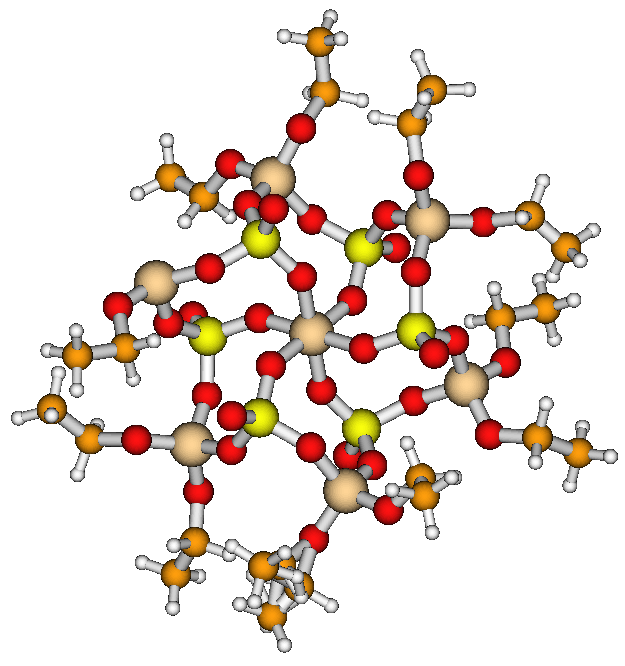
\includegraphics[width=8cm]{rtg_6.png}
%\caption{Výchozí rentgenová struktura \cite{C3NJ00721A};  Legedna: \mycircle{brown} Si, \mycircle{red} O, \mycircle{orange} C,  \mycircle{yellow} P, \mycircleempty{black}~H}
%\label{rtg_6}
%\end{center}
%\end{figure}
V tomto modelu je křemík oblopen šesti fosfáty, které jsou vzájemně zesíťované přes další čtyřkoordinované křemíky. Přítomnost osmičlenného cyklu v silikofosfátech byla potvrzena rentgenovou strukturou \cite{rtg_4_pinkas} a dále podle ní byly vytvářeny cykly v dalších modelech.
\begin{figure}
\begin{center}
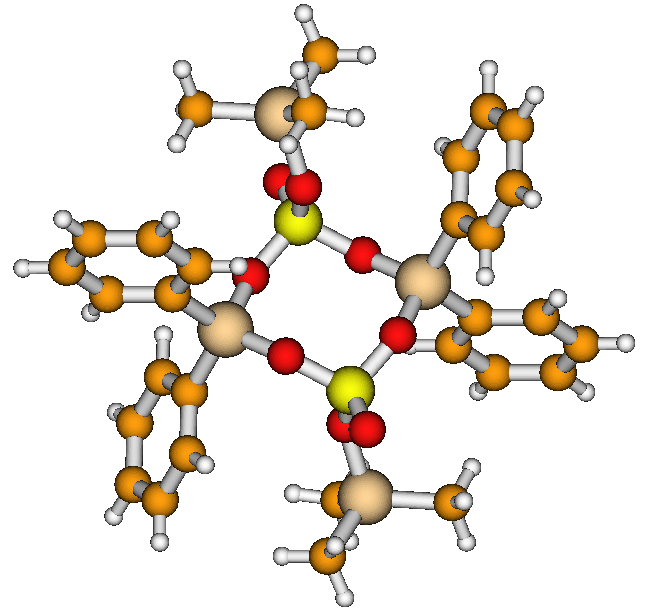
\includegraphics[width=6cm]{rtg_4_kruh_samotne.png}
\caption{Výchozí rentgenová struktura \cite{rtg_4_pinkas};  Legedna: \mycircle{brown} Si, \mycircle{red} O, \mycircle{orange} C, \mycircleempty{black}~H}
\label{rtg_4}
\end{center}
\end{figure}
Z tohoto modelu vycházely všechny ostatní velké struktury se šestikoordinovaným křemíkem. V experimentálních strukturách silikofosfátů byly pozorovány krom fosfátových skupiny také různé acetátové skupiny. Právě přítomnost acetátových skupin měla vliv na chování křemíku a jeho sklon k hypervalenci. Acetátové skupiny se  v okolí křemíku vždy vyskytovaly po dvou a tento jev byl dodržen i v modelových strukturách. Zvolila jsem dvě možnosti umístění acetátových skupin. V prvním případě se acetylové skupiny vůči sobě vyskytovaly v poloze trans \ref{prehled_largeI},  \textbf{R}, ve druhém případě se vysvytovaly v poloze cis \ref{prehled_largeI},  \textbf{Q}.
Při modelování silikofosfátů s acetátovými skupinami v polohách cis a trans jsme vycházeli z uspořádání v původní rentgenové struktuře. Naší snahou bylo zachování původních šesti cyklů. Proto v prvním kole optimalizace bylo ponecháno šest cyklů a dvě fosfátové skupiny nahrazeny acetátovými. Tento model měl problém s vazebným úhlem na atomech 50-11-52 a torzním úhlu na atomech 52 - 11 - 50 - 51 a 50 - 11 - 52 - 54. Jako řešení situace jsme zvolili odstranění dvou cyklů a uvolnění napětí na jednotlivých cyklech. Počet cyklů dva byl zvolen z důvodu zachování symetrie. Uvolněná struktura silikofosfátu s acetáty v poloze trans byla opět optimalizována, tentokrát s pseudopotenciálem z důvodu velikosti struktury. Ve druhém kroku byla provedena optimalizace již s B3LYP/6-31G*. \\
Pro model silikofosfátu s acetátem v poloze cis byla situace obdobná. Výchozí strukturou byl původní model z rtg \ref{prehled_large}, \textbf{O}, kde bylz dva fosfátz nahrazenz acetylz. Toto uspořádání opět vedlo k přílišnému napětí na cyklech a z tohoto důvodu byla provedena stejná operace, jako pro model s acetátem v poloze trans. V modelu silikofofátu s acetátem v poloze cis byly odstraněny nejprve dva cykly a následně ještě jeden, protože struktura stále vykazovala špatné torzní úhly.
Pro strukturu s acetátem v poloze cis bylo nutno odstranit celkově čtyři cykly a výsledný počet cyklů v molekule byl dva. Acetáty byly umístěné v ekvatoriální rovině stejně jako volný fosfát. \\
Další koordinace křemíku, která byla experimentálně pozorována v silikofosfátech byla s křemík v koordinaci pět \ref{prehled_largeI}, \textbf{S}. Tento typ nebyl příliš častý, ale jeho přítomnost je známá z IR. Y tohoto d;vodu jsem také pětikoordinovaný křemík zařadila do analýzy. První návrh struktury silikofosfátu v koordinaci pět byl získán od prof. Pinkase (soukromé sdělení), Ústav Anorganické chemie, MU. Tento model obsahoval křemík v koordinaci pět a celkový počet cyklů byl pět. Toto uspořádání vedlo k špatnému úhlu na atomech 1 - 5 - 9 a větší části špatných torzních úhlů, příkladem může být špatný torní úhel na atomech 3 - 1 - 5 - 9.  Vzhledem k lichému počtu cyklů ve struktuře pětikoordinovaného křemíku byla otázka odstranění cyklů složitější a to především díky snaze zachovat symetrii v systému. Byly zvoleny dva přístupy. První model obsahoval tři cykly a volný fosfát, zde byl špatný vazebný úhel na atomech 1 - 3 - 8. Druhý model obsahoval pouze dva cykly a jeden fosfát, zde došlo k chybě ve vazebném úhlu na atomech 1 - 2 - 7. Nalezení správné struktury s křemíkem v koordinaci pět pomohla rentgenová struktura v článku \cite{rtg_5} \ref{rtg_5}.
\begin{figure}
\begin{center}
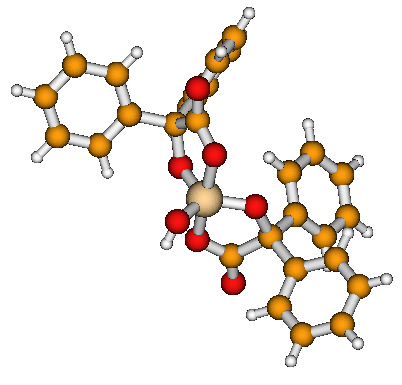
\includegraphics[width=8cm]{rtg_5_koordinace.png}
\caption{Výchozí rentgenové struktury \cite{rtg_5};  Legedna: \mycircle{brown} Si, \mycircle{red} O, \mycircle{orange} C, \mycircleempty{black}~H}
\label{rtg_5}
\end{center}
\end{figure}
Další model pětikoordinovaného křemíku byl inspirován touto rentgenovou strukturou a fosfát byl nahrazen vodíkem. Pro tento model byla udělána výjimka a celkov7 náboj byl snížen z 0 na -1, což se nakonec ukázalo jako vhodné řešení. Původní snaha zachování neutrálního náboje modelových struktur silikofosfátů vycházela z předpokaldu, že samotné amorfní struktury jsou neutrální. V případě pětikoordinovaného křemíku a ale náboj způsobil nerovnoměrnosti v systému. Snížení náboje o jedna vedlo k získání správné struktury s vodíkem, kde se nacházely dvy cykly a jeden volný fosfát. Ve výsledné strukturře byl dočasný vodík nahrazen fosfátem, aby se obnovila původní podoba struktury.

\subsection{Malé modely}
Malé modely podávají podrobnější pohled na charakter vazby Si-C a lze je rozdělit na dvě části. Prní část se věnuje modelovým strukturám, které slouží pro podrobnější analýzu chemické vazby. Druhá část se věnuje výchozím reaktantům, které slouží pro přípravu silikofosfátových polymerů. Obrázky struktur jsou uveden na obrázku \ref{prehled_male_modely}. Pro strukturu \ce{SiCH3(OCH3)5} \ref{prehled_male_modely}, \textbf{C} bylo nutno použit klíčové slovo Opt=CalcFC. Pro sturkturu \ce{Si(OCH3)6} \ref{prehled_male_modely},  \textbf{D} byl použit parametr SCF=Vshift. Model \ce{SiCl4} \ref{prehled_male_modely}, \textbf{E} slouží jako případ sloučeniny, kde křemík není schopen navyšovat koordinaci. Naopak (acetylmethoxyl)trifluorsilan \ref{prehled_male_modely}, \textbf{F} je zde použit jako model, kde je křemík ochoten zvyšovat koordinaci na pět. V tabulce \ref{hsab_small} je shrnutí HSAB analýzy pro malé modely.

\begin{figure}
\centering
\subfigure[\ce{SiCH3(OCH3)3}, \textbf{A}]{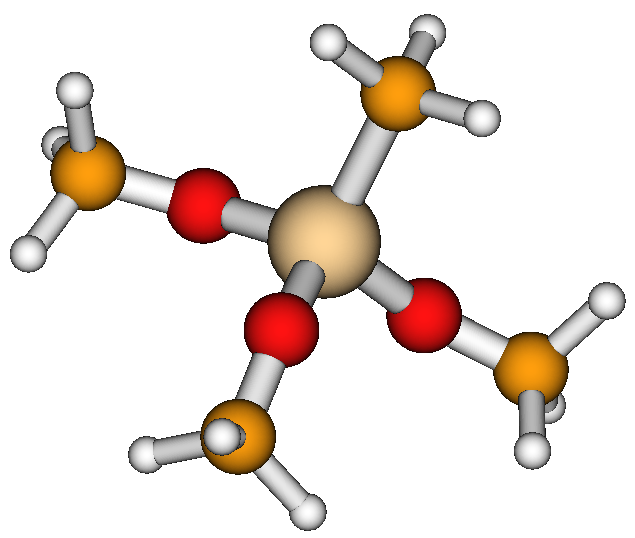
\includegraphics[width=5cm]{si_ch3_och3.png} \label{si_ch3_och3}}
\subfigure[\ce{Si(OCH3)4}, \textbf{B}]{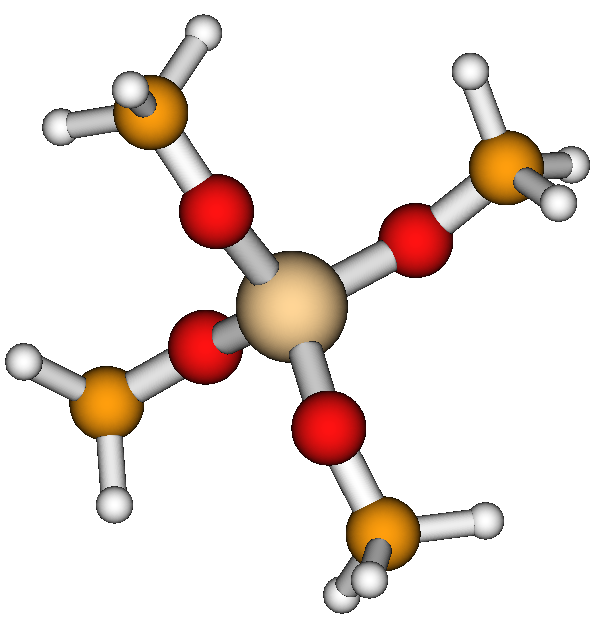
\includegraphics[width=5cm]{si_och3_4.png}\label{si_och3_4}}
\subfigure[\ce{SiCH3(OCH3)5},  \textbf{C}]{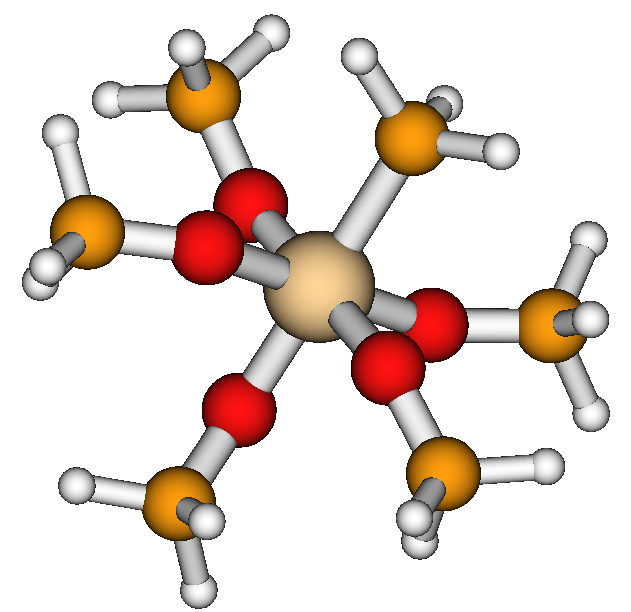
\includegraphics[width=5cm]{si_ch3_och3_5.png}\label{si_ch3_och3_5}}
\subfigure[\ce{Si(OCH3)6},  \textbf{D}]{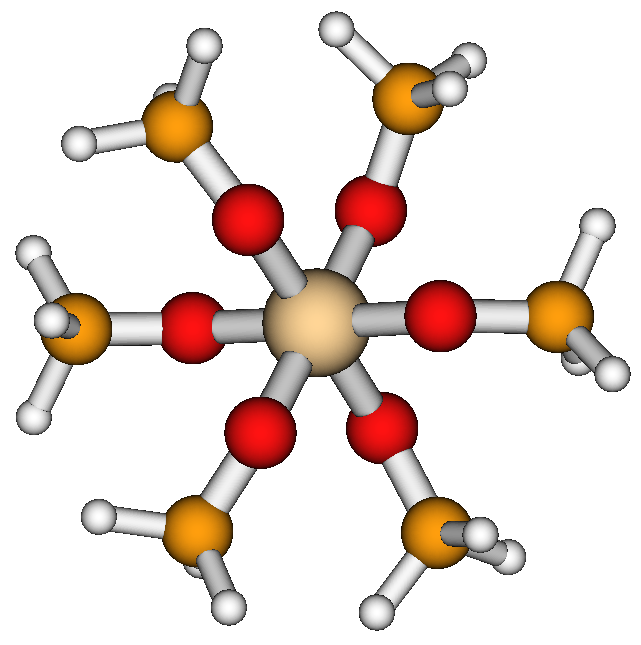
\includegraphics[width=5cm]{si_och3_6.png}\label{si_och3_6}}
\subfigure[\ce{SiCl4},  \textbf{E}]{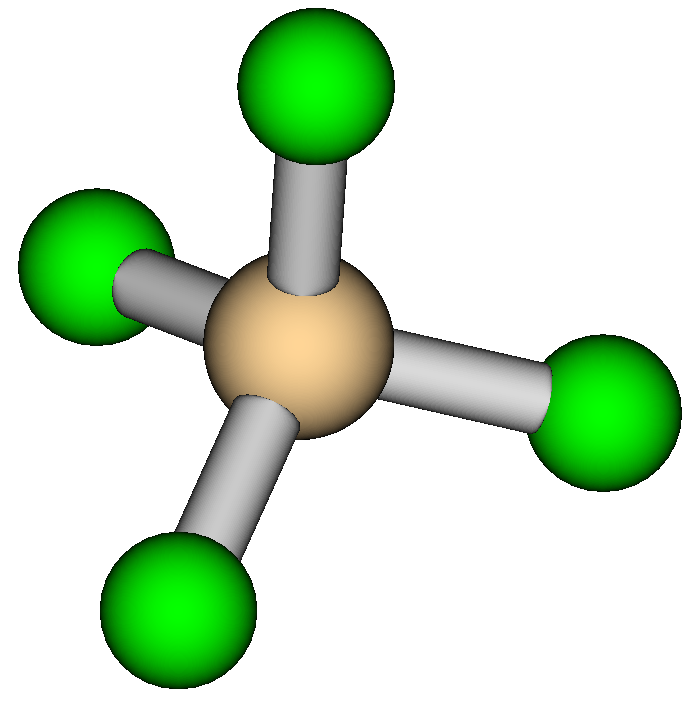
\includegraphics[width=3cm]{si_cl_4.png}\label{si_cl4}}
\subfigure[(acetylmethoxyl)trifluorsilan, \textbf{F}]{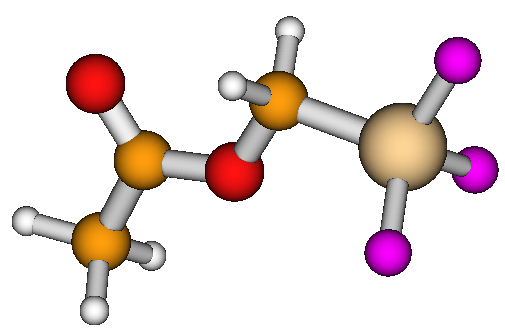
\includegraphics[width=5.5cm]{acetylmethyltriflurosila.png} \label{acetylmethylfluorsilan}}
\caption{Přehled malých struktur; Legedna: \mycircle{brown} Si, \mycircle{red} O, \mycircle{orange} C, \mycircle{green} Cl, \mycircle{red!50!blue!50} F, \mycircleempty{black}~H}
\label{prehled_male_modely}
\end{figure}

\begin{table}[htbp]

\begin{minipage}{\textwidth}
\caption{HSAB analýza malých molekul}
\begin{center}
\begin{tabular}{|l|r|r|r|r|}
\hline
\label{hsab_small}& E$_{\ce{H}}$\footnote{HOMO $-$ \textit{Highest Occupied Molecular Orbital}} [eV] & E$_{\ce{L}}$\footnote{LUMO$ - $\textit{Lowest Unoccupied Molecular Orbital}} [eV]& $\chi$ [eV] & $\eta$ [eV] \\ \hline
\ce{SiCH3(OCH3)3}, \textbf{A} & 3,089 & 10,089 & -6,589 & 3,500 \\ \hline
\ce{Si(OCH3)4}, \textbf{B} & -7,389 & 1,442 & 2,974 & 4,416 \\ \hline
\ce{SiCH3(OCH3)5},  \textbf{C} & 3,089 & 10,089 & -6,589 & 3,500 \\ \hline
\ce{Si(OCH3)6},  \textbf{D} & 3,112 & 9,625 & -6,369 & 3,256 \\ \hline
\ce{SiCl4},  \textbf{E} & -9,770 & -2,221 & 5,995 & 3,774 \\ \hline
(acetylmethoxyl)trifluorsilan, \textbf{F} & -7,825 & -0,066 & 3,946 & 3,880 \\ \hline
\end{tabular}
\end{center}
\end{minipage}
\end{table}

Na základě experimentální práce Aleše Stýskalíka \cite{Styskalik2015thesis} jsem se zabývala křemíkem v koordinaci čtyři, který sloužil jako výchozí reaktant pro přípravu silikofosfátových polymerů.
\begin{figure}
\centering
\subfigure[\ce{Si(OC2H5)4}, \textbf{G}]{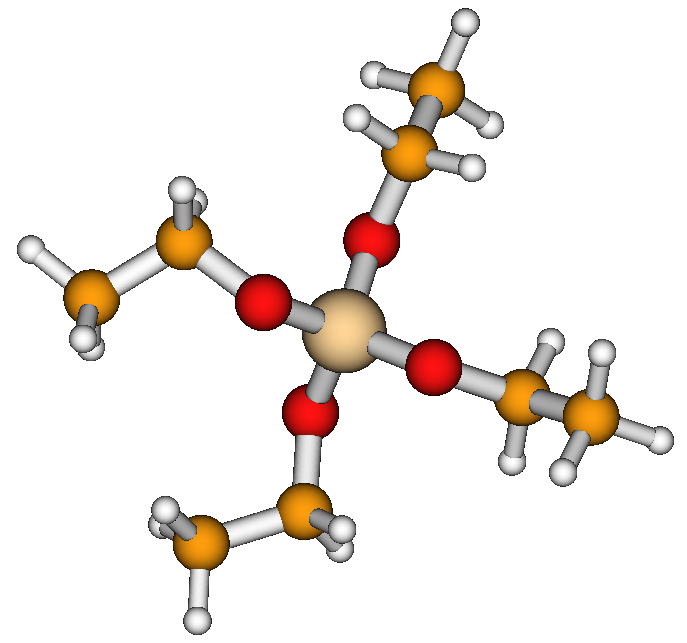
\includegraphics[width=5cm]{si_o_et_4.png} \label{si_oet_4}}
\subfigure[\ce{SiF3(C6H5)},  \textbf{H}]{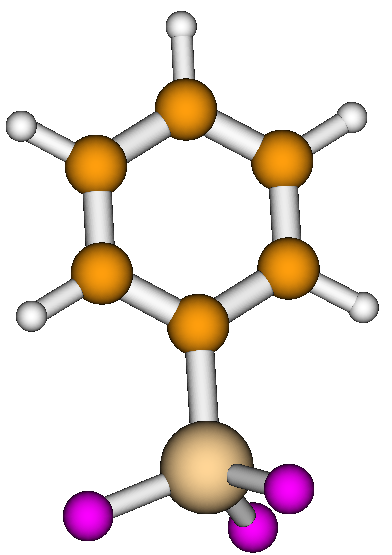
\includegraphics[width=3cm]{si_fenyl_f3.png}\label{si_fenyl_f3}}
\subfigure[\ce{SiCH3(OCOCH3)3},  \textbf{I}]{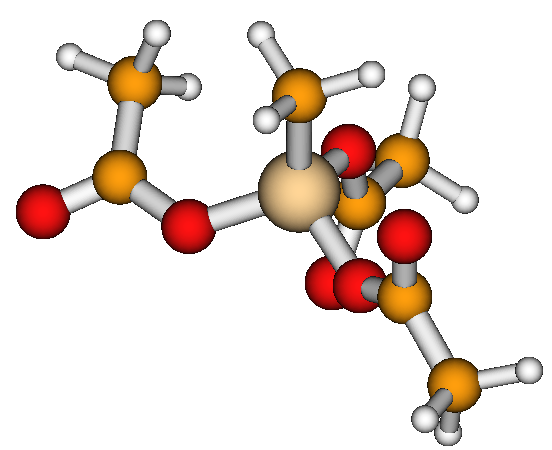
\includegraphics[width=5cm]{si_ch3_oac_3.png}\label{si_ch3_oac_3}}
\subfigure[\ce{SiCH3(OH)3},  \textbf{J}]{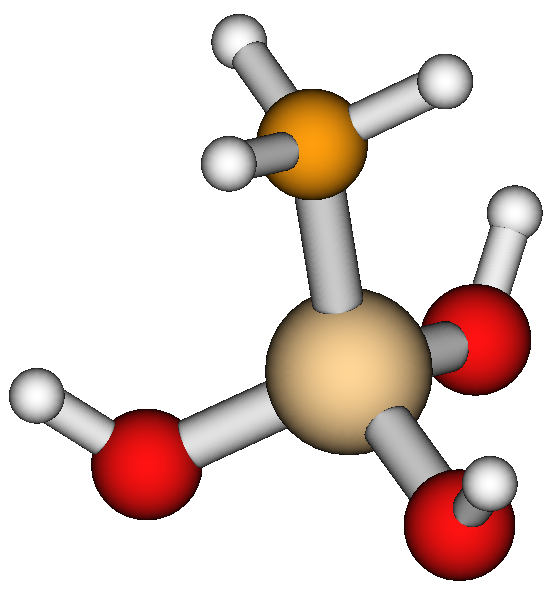
\includegraphics[width=3cm]{si_ch3_och_4.png}\label{si_ch3_och_4}}
\subfigure[\ce{Si(OCOCH3)4},  \textbf{K}]{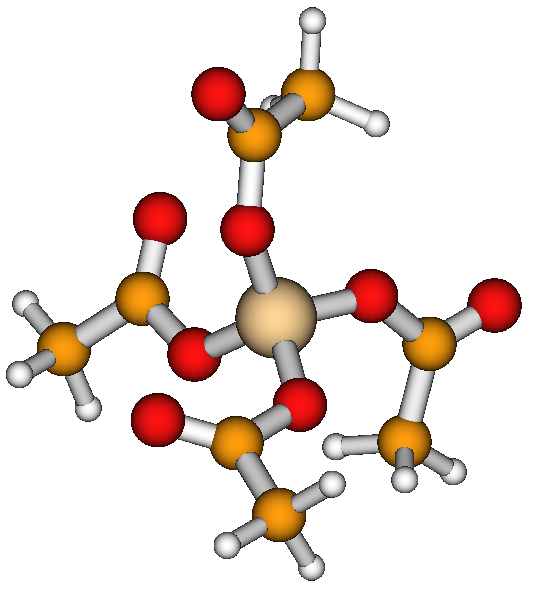
\includegraphics[width=5cm]{si_o_ac_4.png}\label{si_o_ac_4}}
\subfigure[\ce{Si(OCl)(OC2H5)3},  \textbf{L}]{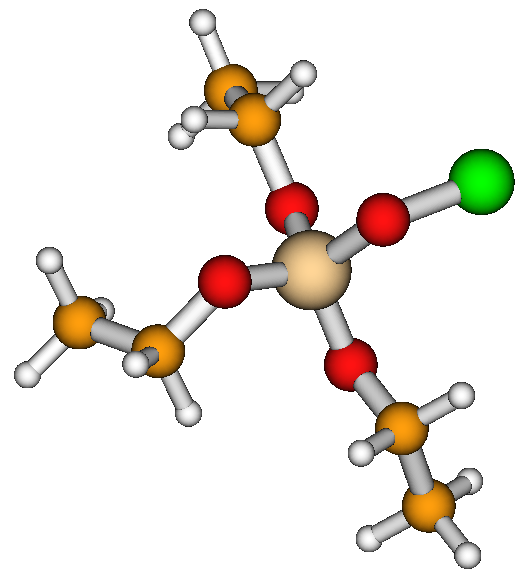
\includegraphics[width=5cm]{si_ocl_oet_3.png}\label{si_ocl_oet_3}}
\caption{Přehled reaktantů; Legedna: \mycircle{brown} Si, \mycircle{red} O, \mycircle{orange} C, \mycircle{red!50!blue!50} F, \mycircle{green}~Cl, \mycircleempty{black}~H}
\label{prehled_male_modely}
\end{figure}


\subsection{Středně velké modely}
Tato část se věňuje nejmenším možným modelům, které již tvoří uvnitř svých struktur cyklus. Přehled struktur je ukázán na obrázku \ref{prehled_middle} Středně velké modely obsahují křemík v koordinaci čtyři a snaží se zachytiti tvorbu cyklů, které vznikají v silikofosfátech. V tabulce \ref{hsab_middle} lze vidět výsledky pro HSAB analýzu.
\begin{figure}
\begin{center}
\subfigure[\ce{SiCH3(PO4(CH3)2)(Si2P2O9(CH3)4)},  \textbf{M}]{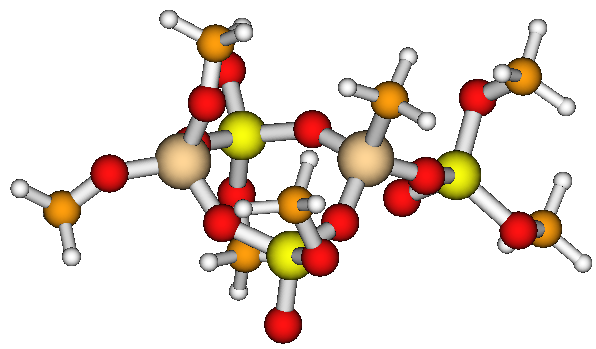
\includegraphics[width=6cm]{si_model_methyl.png}\label{obr_h4sio4_MO_s1_20}}
\subfigure[\ce{Si(Si2P2O9(CH3)4)2}, \textbf{N}]{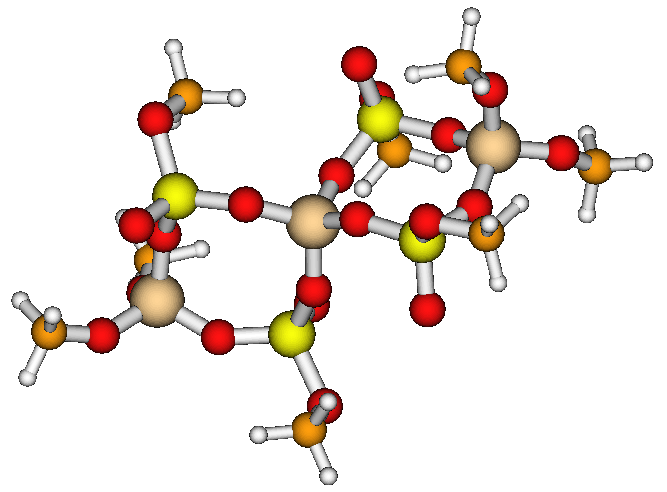
\includegraphics[width=5cm]{si_model_orezany.png}\label{obr_h4sio4_MO_s1_24}}
\caption{Přehled středně velkých modelů];  Legedna: \mycircle{brown} Si, \mycircle{red} O, \mycircle{orange} C, \mycircle{yellow} P, \mycircleempty{black}~H}
\label{prehled_middle}
\end{center}
\end{figure}

\begin{table}[htbp]
\begin{minipage}{\textwidth}
\caption{HSAB analýza středních molekul}
\begin{center}
\begin{tabular}{|l|r|r|r|r|}
\hline
\label{hsab_middle}& E$_{\ce{H}}$\footnote{HOMO $-$ \textit{Highest Occupied Molecular Orbital}} [eV] & E$_{\ce{L}}$\footnote{LUMO$ - $\textit{Lowest Unoccupied Molecular Orbital}} [eV]& $\chi$ [eV] & $\eta$ [eV] \\ \hline
\textbf{M} & -7,802 & 0,494 & 3,654 & 4,148 \\ \hline
\textbf{N} & -8,101 & -0,059 & 4,080 & 4,021 \\ \hline
\end{tabular}
\end{center}
\end{minipage}
\end{table}


\subsection{Velké modely}
Velké modely mají za cíl modelovat vybrané části ze silikofosfátů. Ve svých strukturách už obsahují dva a více cyklů a všechny obsahují křemík v koordinaci šest. Pro velké struktury byla provedena HSAB analýza a výsledky jsou uvedeny v tabulce \ref{hsab_large}. Přehled struktur pro analýzu je uveden na obrázku \ref{prehled_large}.
\begin{figure}
\begin{center}
\caption{Přehled velkých modelů;  Legedna: \mycircle{brown} Si, \mycircle{red} O, \mycircle{orange} C, \mycircle{yellow} P, \mycircleempty{black}~H}
\subfigure[ \textbf{O}]{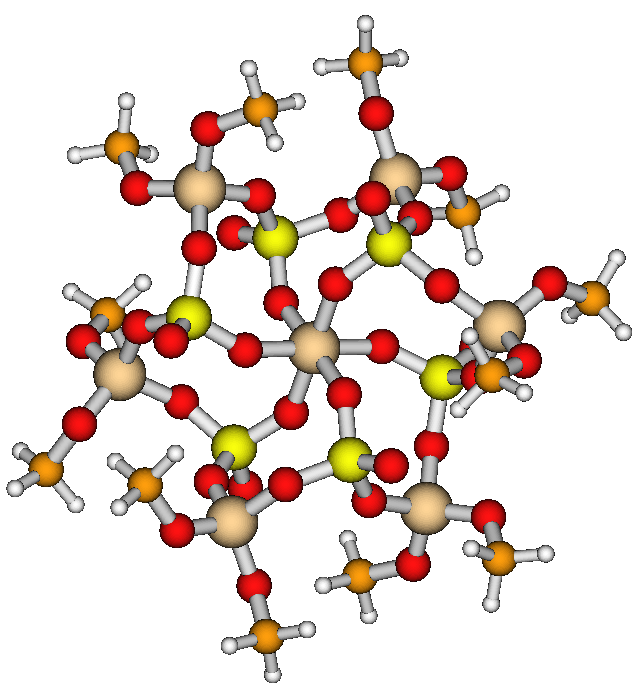
\includegraphics[width=6cm]{struktura_puvodni.png}\label{struktura_puvodni}}
\subfigure[ \textbf{P}]{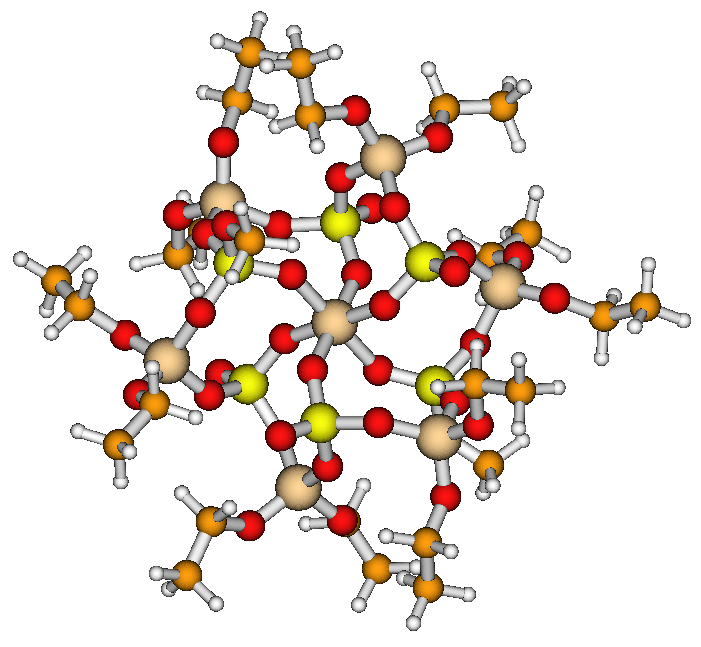
\includegraphics[width=6cm]{srtuktura_bez_naboje.png}\label{struktura_bez_naboje}}
\label{prehled_large}
\end{center}
\end{figure}

\begin{figure}
\begin{center}
\caption{Přehled velkých modelů;  Legedna: \mycircle{brown} Si, \mycircle{red} O, \mycircle{orange} C, \mycircle{yellow} P, \mycircleempty{black}~H}
\subfigure[ \textbf{Q}]{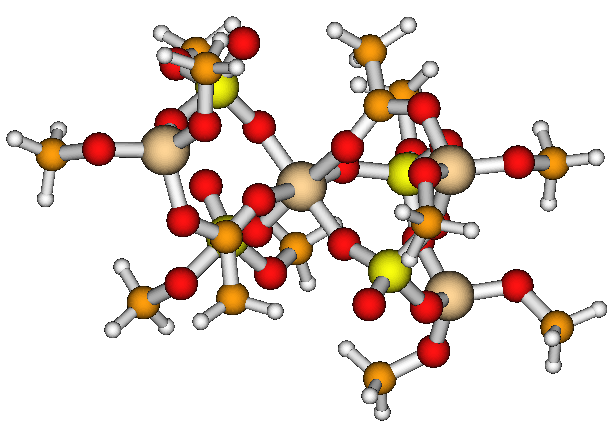
\includegraphics[width=6cm]{struktura_cis.png} \label{struktura_cis}}
\subfigure[ \textbf{R}]{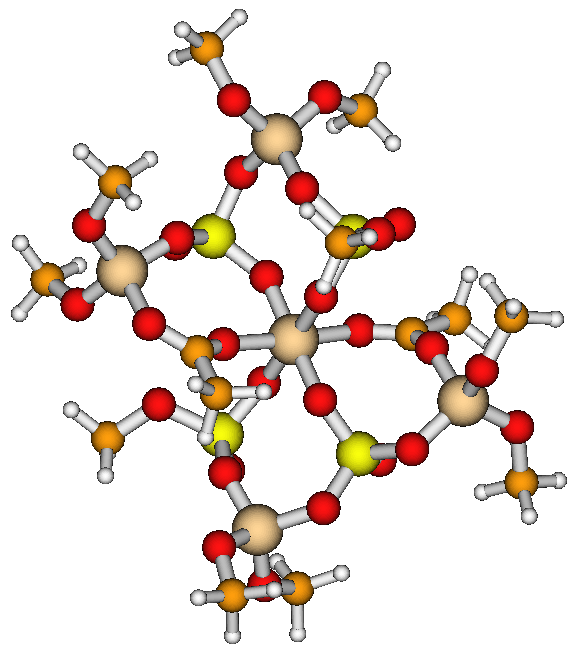
\includegraphics[width=6cm]{struktura_trans.png}\label{struktura_trans}}
\subfigure[ \textbf{S}]{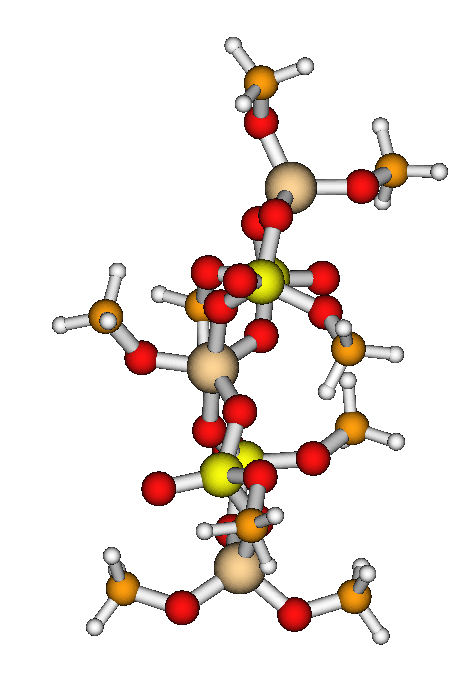
\includegraphics[width=6cm]{strukutra_5_opravena.png}\label{struktura_5}}
\label{prehled_largeI}
\end{center}
\end{figure}

\begin{table}[htbp]
\begin{minipage}{\textwidth}

\caption{HSAB analýza velkých molekul}
\begin{center}
\begin{tabular}{|l|r|r|r|r|}
\hline
\label{hsab_large} & E$_{\ce{H}}$\footnote{HOMO $-$ \textit{Highest Occupied Molecular Orbital}} [eV] & E$_{\ce{L}}$\footnote{LUMO$ - $\textit{Lowest Unoccupied Molecular Orbital}} [eV]& $\chi$ [eV] & $\eta$ [eV] \\ \hline
\textbf{O} & -7,318 & 0,176 & 3,571 & 3,747 \\ \hline
\textbf{P} & -7,351 & -1,392 & 4,372 & 2,980 \\ \hline
\textbf{R} & -7,240 & -1,538 & 4,389 & 2,851 \\ \hline
\textbf{Q} & -2,521 & 5,120 & -1,299 & 3,820 \\ \hline
\textbf{S} & -4,573 & 3,433 & 0,570 & 4,003 \\ \hline
\end{tabular}
\end{center}
\end{minipage}
\end{table}





\section{Vazby}
\renewcommand{\thesubfigure}{(\alph{subfigure})}
Vlastnosti chemických vazeb v silikofosfátech byly modelovány metodou NBO a Mullikenovou populační analýzu. Mullikenova populační analýza(MPA) byla provedena dvěma zůsoby. Pro velké struktury byl počítán orbital LUMO. Pro malé a střední modely byla provedena analýza zdrcadlových orbitalů. \\


\begin{table}[htbp]
\caption{Analýza \ce{SiCH3(OCH3)3}, \textbf{A}}
\begin{center}
\begin{tabular}{|l|r|r|r|r|r|r|r|r|}
\hline
 & 20 & \multicolumn{1}{l|}{} & 33 & \multicolumn{1}{l|}{} & 34 & \multicolumn{1}{l|}{} & 35 & \multicolumn{1}{l|}{} \\ \hline
  & s & p & s & p & s & p & s & p \\ \hline
Si & 11,8\% & 0,2\% & 11,8\% & 9,7\% & 0,2\% & 3,0\% & 3,2\% & 5,4\% \\ \hline
O & 2,3\% & 9,1\% & 2,3\% & 17,4\% & 0,4\% & 26,0\% & 26,5\% & 34,0\% \\ \hline
O & 2,5\% & 8,0\% & 2,5\% & 19,7\% & 0,8\% & 16,7\% & 17,5\% & 20,7\% \\ \hline
O & 2,2\% & 9,0\% & 2,2\% & 16,5\% & 0,4\% & 24,3\% & 24,7\% & 17,1\% \\ \hline
C & 1,7\% & 4,9\% & 1,7\% & 2,5\% & 0,1\% & 1,5\% & 1,6\% & 1,5\% \\ \hline
\end{tabular}
\end{center}
\label{si_ch3_och3_MPA}
\end{table}

\begin{table}[htbp]
\caption{Analýza LUMO pro \ce{SiCH3(OCH3)5},  \textbf{C}}
\begin{center}
\begin{tabular}{|l|r|r|}
\hline
 & \multicolumn{1}{l|}{S} & \multicolumn{1}{l|}{P} \\ \hline
Si & 0,2\% & 0,5\% \\ \hline
O & 1,7\% & 0,1\% \\ \hline
O & 1,3\% & 0,1\% \\ \hline
O & 0,2\% & 0,1\% \\ \hline
O & 0,9\% & 0,1\% \\ \hline
O & 2,5\% & 0,4\% \\ \hline
C & 58,9\% & 0,1\% \\ \hline
\end{tabular}
\end{center}
\label{si_ch3_och3_5_MPA}
\end{table}

\begin{table}[htbp]
\caption{Analýza LUMO pro \ce{Si(OCH3)6}, \textbf{D}}
\begin{center}
\begin{tabular}{|l|r|r|}
\hline
 & \multicolumn{1}{l|}{S} & \multicolumn{1}{l|}{P} \\ \hline
Si & 2,0\% & 0,0\% \\ \hline
O & 0,1\% & 0,1\% \\ \hline
O & 0,1\% & 0,1\% \\ \hline
O & 0,1\% & 0,1\% \\ \hline
O & 0,1\% & 0,1\% \\ \hline
O & 0,1\% & 0,1\% \\ \hline
C & 0,1\% & 0,1\% \\ \hline
\end{tabular}
\end{center}
\label{si_och3_6_MPA}
\end{table}

\begin{table}[htbp]
\caption{Analýza \ce{Si(OCH3)4}, \textbf{B}}
\begin{center}
\begin{tabular}{|l|r|r|r|r|r|r|r|r|}
\hline
& 22 & \multicolumn{1}{l|}{} & 35 & \multicolumn{1}{l|}{} & 36 & \multicolumn{1}{l|}{} & 37 & \multicolumn{1}{l|}{} \\ \hline
 & \multicolumn{1}{l|}{S} & \multicolumn{1}{l|}{P} & \multicolumn{1}{l|}{S} & \multicolumn{1}{l|}{P} & \multicolumn{1}{l|}{S} & \multicolumn{1}{l|}{P} & \multicolumn{1}{l|}{S} & \multicolumn{1}{l|}{P} \\ \hline
Si & 11,10 \% & 0,0\% & 0,0\% & 12,3\% & 0,0\% & 12,3\% & 0,0\% & 2,7\% \\ \hline
O & 2,50 \% & 5,4\% & 1,7\% & 9,4\% & 3,8\% & 9,3\% & 0,2\% & 15,4\% \\ \hline
O & 2,50 \% & 5,4\% & 3,8\% & 9,3\% & 1,7\% & 9,4\% & 0,2\% & 15,4\% \\ \hline
O & 2,50 \% & 5,4\% & 1,7\% & 9,4\% & 3,8\% & 9,3\% & 0,2\% & 15,4\% \\ \hline
C & 2,50 \% & 5,4\% & 3,8\% & 9,3\% & 1,7\% & 9,4\% & 0,2\% & 15,4\% \\ \hline
\end{tabular}
\end{center}
\label{si_och3_4_MPA}
\end{table}

\begin{table}[htbp]
\caption{Analýza acetylmethyltrifluorsilan, \textbf{F}}
\begin{center}
\begin{tabular}{|l|r|r|r|r|r|r|r|r|}
\hline
& 22 & \multicolumn{1}{l|}{} & 25 & \multicolumn{1}{l|}{} & 26 & \multicolumn{1}{l|}{} & 27 & \multicolumn{1}{l|}{} \\ \hline
 & \multicolumn{1}{l|}{S} & \multicolumn{1}{l|}{P} & \multicolumn{1}{l|}{S} & \multicolumn{1}{l|}{P} & \multicolumn{1}{l|}{S} & \multicolumn{1}{l|}{P} & \multicolumn{1}{l|}{S} & \multicolumn{1}{l|}{P} \\ \hline\textbf{Si} & 17,9\% & 0,2\% & 0,3\% & 8,9\% & 0,0\% & 6,9\% & 0,9\% & 7,5\% \\ \hline
\textbf{F} & 4,3\% & 9,0\% & 3,4\% & 22,2\% & 0,0\% & 6,7\% & 1,9\% & 13,6\% \\ \hline
\textbf{F} & 5,4\% & 9,9\% & 1,5\% & 12,6\% & 3,3\% & 19,6\% & 0,1\% & 6,8\% \\ \hline
\textbf{F} & 5,4\% & 9,9\% & 1,5\% & 12,6\% & 3,3\% & 19,6\% & 0,1\% & 6,8\% \\ \hline
\textbf{C} & 2,6\% & 4,9\% & 0,9\% & 0,9\% & 0,0\% & 0,5\% & 0,7\% & 1,8\% \\ \hline
\end{tabular}
\end{center}
\label{acetylmethyltrifluorsilan_MPA}
\end{table}


\begin{table}[htbp]
\caption{Analýza \ce{SiCH3(PO4(CH3)2)(Si2P2O9(CH3)4)},  \textbf{M}}
\begin{center}
\begin{tabular}{|l|r|r|r|r|r|r|r|r|}
\hline
 & 61 & \multicolumn{1}{l|}{} & 68 & \multicolumn{1}{l|}{} & 70 & \multicolumn{1}{l|}{} & 106 & \multicolumn{1}{l|}{} \\ \hline
  & \multicolumn{1}{l|}{S} & \multicolumn{1}{l|}{P} & \multicolumn{1}{l|}{S} & \multicolumn{1}{l|}{P} & \multicolumn{1}{l|}{S} & \multicolumn{1}{l|}{P} & \multicolumn{1}{l|}{S} & \multicolumn{1}{l|}{P} \\ \hline
SI  & 4,2\% & 0,1\% & 4,3\% & 0,4\% & 3,9\% & 0,5\% & 0,9\% & 1,2\% \\ \hline
O & 0,0\% & 2,2\% & 0,2\% & 2,4\% & 0,1\% & 11,4\% & 0,6\% & 3,3\% \\ \hline
O & 0,1\% & 1,5\% & 0,1\% & 5,5\% & 0,2\% & 2,7\% & 0,0\% & 12,9\% \\ \hline
O & 0,0\% & 2,1\% & 0,2\% & 6,6\% & 0,8\% & 0,6\% & 0,0\% & 13,4\% \\ \hline
C & 19,7\% & 5,8\% & 6,7\% & 14,9\% & 1,8\% & 15,2\% & 3,0\% & 31,6\% \\ \hline
\end{tabular}
\end{center}
\label{si_model_methyl_MPA}
\end{table}

\begin{table}[htbp]
\caption{Analýza \ce{Si(Si2P2O9(CH3)4)2}, \textbf{N}}
\begin{center}
\begin{tabular}{|l|r|r|r|r|r|r|r|r|}
\hline
 & 61 & \multicolumn{1}{l|}{} & 68 & \multicolumn{1}{l|}{} & 70 & \multicolumn{1}{l|}{} & 106 & \multicolumn{1}{l|}{} \\ \hline
  & \multicolumn{1}{l|}{S} & \multicolumn{1}{l|}{P} & \multicolumn{1}{l|}{S} & \multicolumn{1}{l|}{P} & \multicolumn{1}{l|}{S} & \multicolumn{1}{l|}{P} & \multicolumn{1}{l|}{S} & \multicolumn{1}{l|}{P} \\ \hline
SI  & 0,0\% & 0,00 \% & 2,8\% & 0,01 \% & 0,0\% & 0,05 \% & 0,0\% & 0,05 \% \\ \hline
O & 0,0\% & 0,00 \% & 13,4\% & 0,49 \% & 2,5\% & 0,09 \% & 0,1\% & 1,14 \% \\ \hline
O & 0,0\% & 0,00 \% & 10,1\% & 0,28 \% & 0,8\% & 0,02 \% & 0,2\% & 0,36 \% \\ \hline
O & 0,0\% & 0,00 \% & 7,9\% & 0,25 \% & 0,3\% & 0,02 \% & 0,0\% & 0,04 \% \\ \hline
O & 0,0\% & 0,00 \% & 6,9\% & 0,19 \% & 0,5\% & 0,02 \% & 0,0\% & 0,07 \% \\ \hline
\end{tabular}
\end{center}
\label{si_model_orezany_MPA}
\end{table}

\begin{table}[htbp]
  \begin{minipage}{\textwidth}
\caption{Výsledky NBO pro malé modely.}
\begin{center}
  \begin{tabular}{|l|l|l|r|r|r|r|r|r|}
  \hline
  \label{nbo_small} &  & Vazba & O.Č\footnote{Obsazovací číslo křemíku} & Si & X\footnote{Procenta druhého atomu ve vazbe} & Si(s) & Si(p) &Si(d) \\ \hline
\textbf{A} & Si-O & 1-2  & 0,066 & 88,3\% & 11,7\% & 23,9\% & 51,9\% & 24,2\% \\ \hline
   &  & 1-3 & 0,111 & 86,5\% & 13,5\% & 23,2\% & 73,3\% & 3,5\% \\ \hline
   &  & 1-3 & 0,092 & 97,1\% & 2,9\% & 0,2\% & 56,7\% & 43,3\% \\ \hline
   &  & 1-4 & 0,065 & 88,5\% & 11,5\% & 23,6\% & 50,2\% & 26,2\% \\ \hline
   & Si-C & 1-17 & 0,073 & 75,5\% & 24,5\% & 29,3\% & 68,9\% & 1,8\% \\ \hline
  \textbf{B} & Si-O &  & 0,104 & 86,1\% & 13,9\% & 25,0\% & 71,4\% & 3,6\% \\ \hline
 \textbf{C} & Si-O & 1-2  & 0,100 & 92,1\% & 7,9\% & 16,0\% & 50,0\% & 33,9\% \\ \hline
   &  & 1-3 & 0,104 & 91,9\% & 8,1\% & 15,0\% & 50,6\% & 34,4\% \\ \hline
   &  & 1-4 & 0,096 & 91,9\% & 8,1\% & 16,5\% & 50,4\% & 33,1\% \\ \hline
   &  & 1-5 & 0,095 & 91,9\% & 8,1\% & 16,4\% & 50,6\% & 33,0\% \\ \hline
   &  & 1-6 & 0,103 & 92,1\% & 7,9\% & 16,1\% & 50,1\% & 33,8\% \\ \hline
   & Si-C & 1-27 & 0,068 & 84,6\% & 15,4\% & 22,8\% & 51,2\% & 26,1\% \\ \hline
  \textbf{D} & Si-O &  & 0,098 & 91,8\% & 8,2\% & 16,7\% & 50,0\% & 33,3\% \\ \hline
  \textbf{E} & Si-Cl & 1-2  & 0,141 & 74,0\% & 26,0\% & 25,0\% & 72,4\% & 2,6\% \\ \hline
   &  & 1-3 & 0,141 & 74,0\% & 26,0\% & 25,0\% & 72,4\% & 2,6\% \\ \hline
   &  & 1-4 & 0,141 & 74,0\% & 26,0\% & 25,0\% & 72,4\% & 2,6\% \\ \hline
   &  & 1-5 & 0,141 & 74,0\% & 26,0\% & 25,0\% & 72,4\% & 2,6\% \\ \hline
  \textbf{F}  & Si-F &1-2 &0,107 & 87,1\% & 12,9\% & 22,5\% & 75,6\% & 2,0\% \\ \hline
 & Si-F &1-3 & 0,107 & 87,1\% & 13,0\% & 22,7\% & 75,4\% & 1,9\% \\ \hline
 & Si-F &1-4 &0,107 & 87,1\% & 13,0\% & 22,7\% & 75,4\% & 1,9\% \\ \hline
 & Si-C &1-5 &0,079 & 74,3\% & 25,7\% & 32,2\% & 65,8\% & 2,0\% \\ \hline
  \end{tabular}
\end{center}
\end{minipage}
\end{table}

\begin{table}[htbp]
  \begin{minipage}{\textwidth}
\caption{Výsledky NBO pro středně velké modely.}
\begin{tabular}{|l|l|l|r|r|r|r|r|r|}
  \hline
  \label{nbo_small} &  & Vazba & O.Č\footnote{Obsazovací číslo křemíku} & Si & X\footnote{Procenta druhého atomu ve vazbe} & Si(s) & Si(p) &Si(d) \\ \hline
\textbf{M} & Si-O & 1-2 & 0,087 & 87,5\% & 12,5\% & 23,8\% & 73,1\% & 3,1\% \\ \hline
 & Si-O & 1-3 & 0,093 & 87,3\% & 12,7\% & 23,0\% & 73,5\% & 3,6\% \\ \hline
 & Si-O & 1-4 & 0,094 & 87,5\% & 12,5\% & 22,6\% & 73,9\% & 3,4\% \\ \hline
 & Si-C & 1-5 & 0,065 & 74,1\% & 25,9\% & 30,7\% & 67,7\% & 1,6\% \\ \hline
\textbf{N} & Si-O & 1-2 & 0,086 & 87,1\% & 12,9\% & 25,7\% & 71,1\% & 3,3\% \\ \hline
 & Si-O & 1-3 & 0,104 & 87,4\% & 12,6\% & 23,9\% & 72,5\% & 3,6\% \\ \hline
 & Si-O & 1-4 & 0,098 & 87,2\% & 12,8\% & 24,6\% & 71,9\% & 3,5\% \\ \hline
 & Si-O & 1-5 & 0,092 & 86,8\% & 13,2\% & 25,8\% & 70,8\% & 3,4\% \\ \hline
\end{tabular}
\end{minipage}
\end{table}




\begin{table}[htbp]
\caption{Analýza \textbf{P}, původní struktura bez náboje, \ref{struktura_bez_naboje}}
\begin{center}
\begin{tabular}{|l|r|r|}
\hline
 & \multicolumn{1}{l|}{S} & \multicolumn{1}{l|}{P} \\ \hline
Si & 9,6\% & 0,01 \% \\ \hline
O & 3,2\% & 0,35 \% \\ \hline
O & 7,5\% & 2,35 \% \\ \hline
O & 3,7\% & 0,36 \% \\ \hline
O & 3,4\% & 0,19 \% \\ \hline
O & 6,7\% & 2,05 \% \\ \hline
O & 3,4\% & 0,37 \% \\ \hline
\end{tabular}
\end{center}
\label{struktura_bez_naboje_MPA}
\end{table}

\begin{table}[htbp]
\caption{Analýza \textbf{Q}, acetáty v poloze cis, \ref{struktura_cis}}
\begin{center}
\begin{tabular}{|l|r|r|}
\hline
 & \multicolumn{1}{l|}{S} & \multicolumn{1}{l|}{P} \\ \hline
Si & 3,1\% & 0,92 \% \\ \hline
O & 0,0\% & 7,59 \% \\ \hline
O & 0,3\% & 0,25 \% \\ \hline
O & 0,9\% & 0,58 \% \\ \hline
O & 0,5\% & 0,08 \% \\ \hline
O & 0,1\% & 18,81 \% \\ \hline
O & 0,5\% & 0,19 \% \\ \hline
\end{tabular}
\end{center}
\label{struktura_C_cis_MPA}
\end{table}

\begin{table}[htbp]
\caption{Analýza struktura pětikoordinovaný \textbf{S}, \ref{struktura_5}}
\begin{center}
\begin{tabular}{|l|r|r|}
\hline
 & \multicolumn{1}{l|}{S} & \multicolumn{1}{l|}{P} \\ \hline
 Si & 23,5\% & 1,72 \% \\ \hline
 O & 5,6\% & 0,95 \% \\ \hline
 O & 12,7\% & 1,06 \% \\ \hline
 O & 7,3\% & 0,81 \% \\ \hline
 O & 13,3\% & 2,16 \% \\ \hline
 O & 2,8\% & 2,05 \% \\ \hline
\end{tabular}
\end{center}
\label{struktura_5_MPA}
\end{table}

\begin{table}[htbp]
\caption{Analýza \textbf{R}, acetáty v poloze trans, \ref{struktura_trans}}
\begin{center}
\begin{tabular}{|l|r|r|}
\hline
 & \multicolumn{1}{l|}{S} & \multicolumn{1}{l|}{P} \\ \hline
Si & 0,5\% & 4,04 \% \\ \hline
O & 0,9\% & 0,33 \% \\ \hline
O & 0,1\% & 8,38 \% \\ \hline
O & 0,1\% & 0,17 \% \\ \hline
O & 0,0\% & 20,85 \% \\ \hline
O & 1,4\% & 0,65 \% \\ \hline
O & 0,7\% & 0,15 \% \\ \hline
\end{tabular}
\end{center}
\label{struktura_C_trans_MPA}
\end{table}

\begin{table}[htbp]
\caption{Analýza \textbf{O}, původní RTG struktura \ref{struktura_puvodni}}
\begin{center}
\begin{tabular}{|l|r|r|}
\hline
 & \multicolumn{1}{l|}{S} & \multicolumn{1}{l|}{P} \\ \hline
Si & 8,8\% & 0,00 \% \\ \hline
O & 3,5\% & 0,36 \% \\ \hline
O & 4,7\% & 0,65 \% \\ \hline
O & 4,1\% & 0,51 \% \\ \hline
O & 4,1\% & 0,42 \% \\ \hline
O & 3,9\% & 0,49 \% \\ \hline
O & 3,9\% & 0,37 \% \\ \hline
\end{tabular}
\end{center}
\label{struktura_puvodni_MPA}
\end{table}


\begin{table}
\caption{Výsledky NBO pro velké modely}
\begin{minipage}{\textwidth}
\begin{center}
\begin{tabular}{|l|l|l|r|r|r|r|r|r|}
\hline
 \label{nbo_large}&  & Vazba & O.Č\footnote{Obsazovací číslo křemíku} & Si & X\footnote{Procenta druhého atomu ve vazbe} & Si(s) & Si(p) &Si(d) \\ \hline
A & Si-O & 1-2  & 0,089 & 91,33 \% & 8,67 \% & 17,15 \% & 49,89 \% & 32,96 \% \\ \hline
 &  & 1-3  & 0,105 & 92,66 \% & 7,34 \% & 16,06 \% & 50,23 \% & 33,72 \% \\ \hline
 &  & 1-4  & 0,088 & 91,24 \% & 8,76 \% & 17,21 \% & 50,07 \% & 32,72 \% \\ \hline
 &  & 1-5  & 0,089 & 91,48 \% & 8,52 \% & 16,70 \% & 50,16 \% & 33,13 \% \\ \hline
 &  & 1-6 & 0,104 & 92,53 \% & 7,47 \% & 16,29 \% & 49,80 \% & 33,91 \% \\ \hline
 &  & 1-7 & 0,088 & 91,29 \% & 8,71 \% & 16,98 \% & 49,95 \% & 33,08 \% \\ \hline
B & Si-O & 1-3  & 0,175 & 89,18 \% & 10,82 \% & 31,84 \% & 64,07 \% & 4,08 \% \\ \hline
 &  & 1-4  & 0,171 & 88,78 \% & 11,22 \% & 33,01 \% & 63,00 \% & 4,00 \% \\ \hline
 &  & 1-5  & 0,132 & 88,88 \% & 11,12 \% & 16,88 \% & 79,32 \% & 3,80 \% \\ \hline
 &  & 1-7 & 0,127 & 88,94 \% & 11,06 \% & 16,73 \% & 79,55 \% & 3,72 \% \\ \hline
C & Si-O & 1-2  & 0,106 & 90,65 \% & 9,35 \% & 22,30 \% & 52,16 \% & 25,54 \% \\ \hline
 &  & 1-4  & 0,113 & 90,69 \% & 9,31 \% & 22,02 \% & 51,83 \% & 26,15 \% \\ \hline
 &  & 1-5  & 0,161 & 90,48 \% & 9,52 \% & 9,91 \% & 86,47 \% & 3,62 \% \\ \hline
 &  & 1-6 & 0,111 & 90,57 \% & 9,43 \% & 21,86 \% & 52,57 \% & 25,57 \% \\ \hline
 &  & 1-7 & 0,104 & 90,19 \% & 9,43 \% & 23,30 \% & 51,81 \% & 24,89 \% \\ \hline
D & Si-O & 1-2  & 0,092 & 91,57 \% & 8,43 \% & 16,92 \% & 50,05 \% & 33,03 \% \\ \hline
 &  & 1-3  & 0,094 & 91,82 \% & 8,18 \% & 16,49 \% & 50,05 \% & 33,46 \% \\ \hline
 &  & 1-4  & 0,092 & 91,67 \% & 8,33 \% & 16,73 \% & 49,90 \% & 33,37 \% \\ \hline
 &  & 1-5  & 0,093 & 91,74 \% & 8,26 \% & 16,54 \% & 49,96 \% & 33,50 \% \\ \hline
 &  & 1-6 & 0,093 & 91,73 \% & 8,27 \% & 16,72 \% & 49,96 \% & 33,32 \% \\ \hline
 &  & 1-7 & 0,093 & 91,75 \% & 8,25 \% & 16,59 \% & 50,11 \% & 33,30 \% \\ \hline
E & Si-O & 1-2  & 0,091 & 91,63 \% & 8,37 \% & 17,13 \% & 50,11 \% & 32,76 \% \\ \hline
 &  & 1-3  & 0,115 & 89,41 \% & 10,59 \% & 20,87 \% & 63,97 \% & 15,16 \% \\ \hline
 &  & 1-4  & 0,085 & 91,53 \% & 8,47 \% & 17,31 \% & 50,82 \% & 31,88 \% \\ \hline
 &  & 1-5  & 0,113 & 90,01 \% & 9,99 \% & 20,02 \% & 62,64 \% & 17,34 \% \\ \hline
 &  & 1-6 & 0,093 & 86,99 \% & 13,01 \% & 24,67 \% & 65,85 \% & 9,48 \% \\ \hline
\end{tabular}\end{center}\end{minipage}\end{table}

\begin{figure}
\begin{center}
\caption{Přehled NBO pro \ce{Si(CH3)(OAC)3};  Legedna: \mycircle{black!50!white!50} Si, \mycircle{red} O, \mycircle{black} C, \mycircle{yellow} P, \mycircleempty{black}~H}
\subfigure[Si 0,06087]{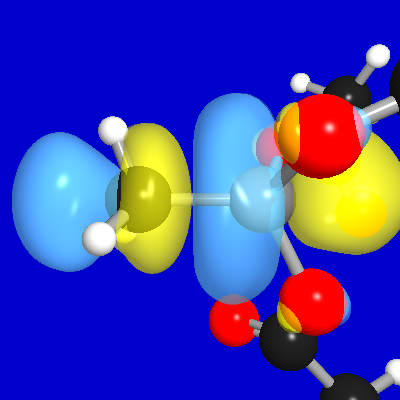
\includegraphics[width=6cm]{si_ch3_59.png} \label{}}
\subfigure[Si 0,10861]{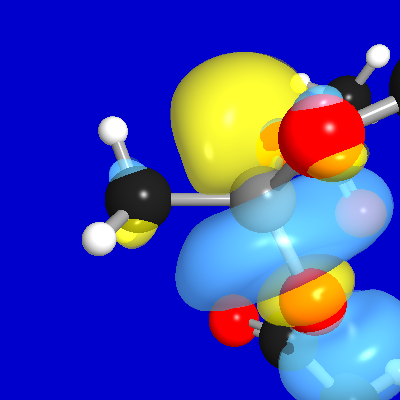
\includegraphics[width=6cm]{si_ch3_63.png}\label{}}
\subfigure[Si 0,08923]{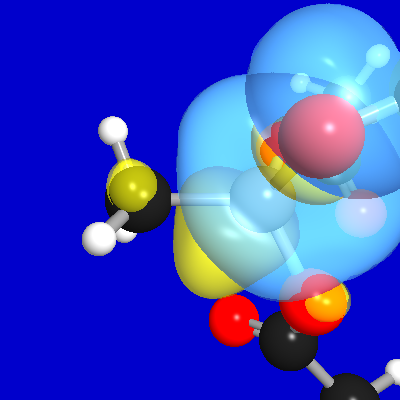
\includegraphics[width=6cm]{si_ch3_64.png}\label{}}
\subfigure[Si 0,07864]{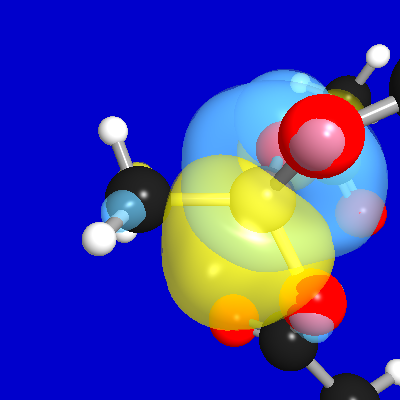
\includegraphics[width=6cm]{si_ch3_65.png}\label{}}
\label{prehled_nbo_si_ch3_oac_3}
\end{center}
\end{figure}

\begin{figure}
\begin{center}
\caption{Přehled NBO pro \ce{Si(OAC)4};  Legedna: \mycircle{black!50!white!50} Si, \mycircle{red} O, \mycircle{black} C, \mycircle{yellow} P, \mycircleempty{black}~H}
\subfigure[Si 0,10831]{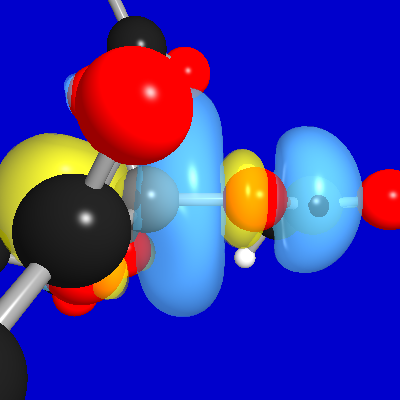
\includegraphics[width=6cm]{SI_AC_70.png} \label{}}
\subfigure[Si 0,11457]{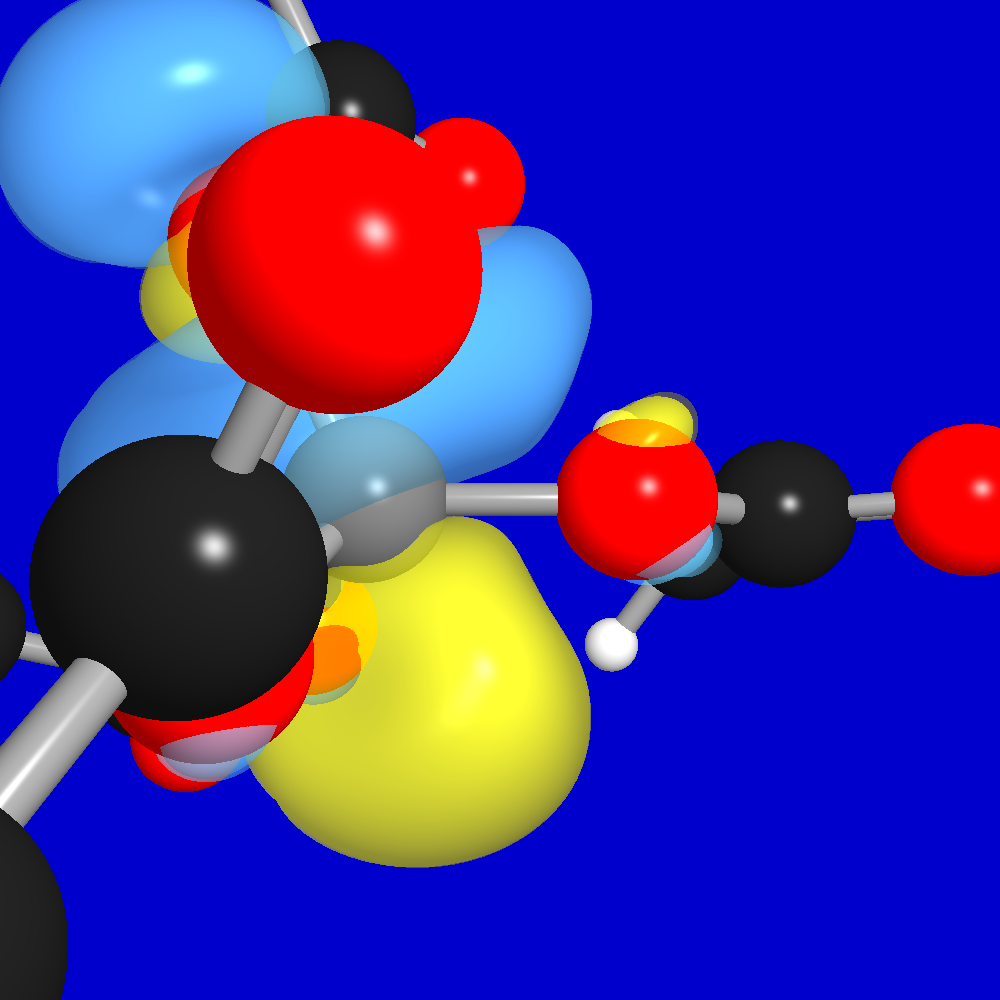
\includegraphics[width=6cm]{SI_AC_71.png}\label{}}
\subfigure[Si 0,11286]{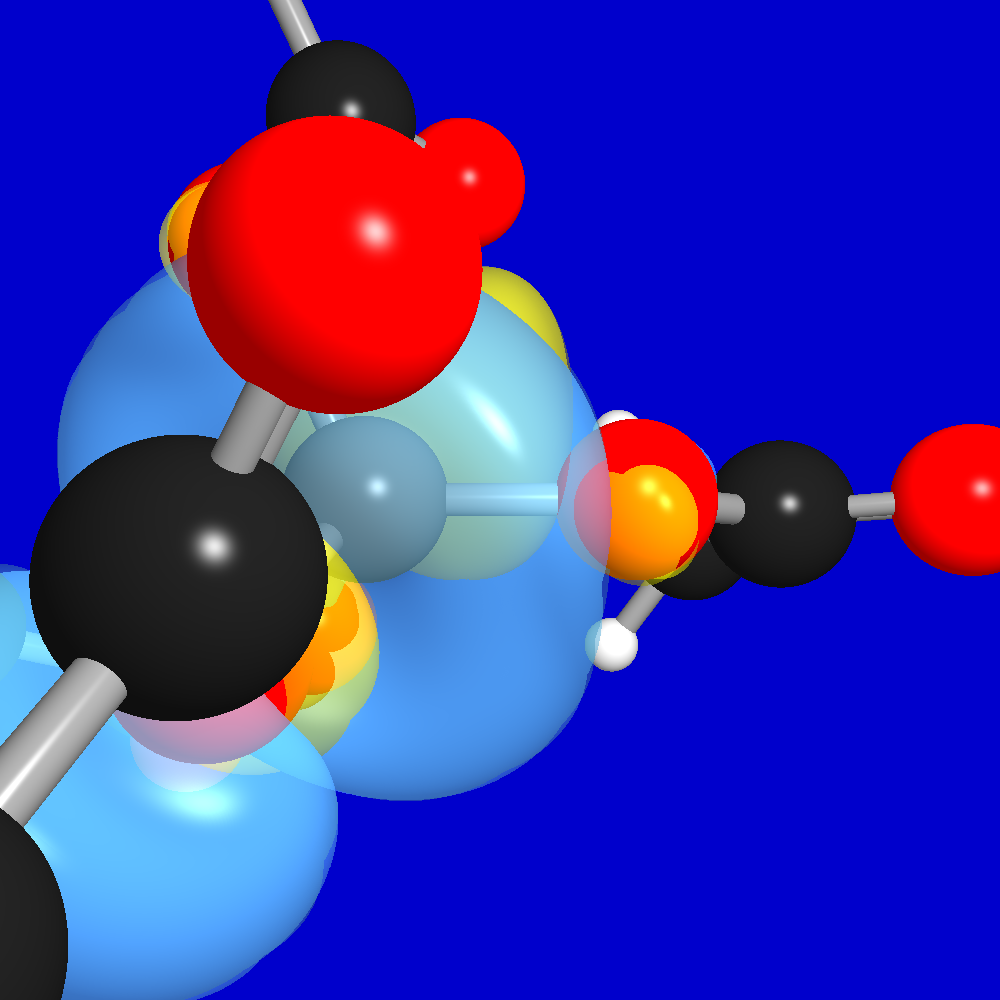
\includegraphics[width=6cm]{SI_AC_72.png}\label{}}
\subfigure[Si 0,10636]{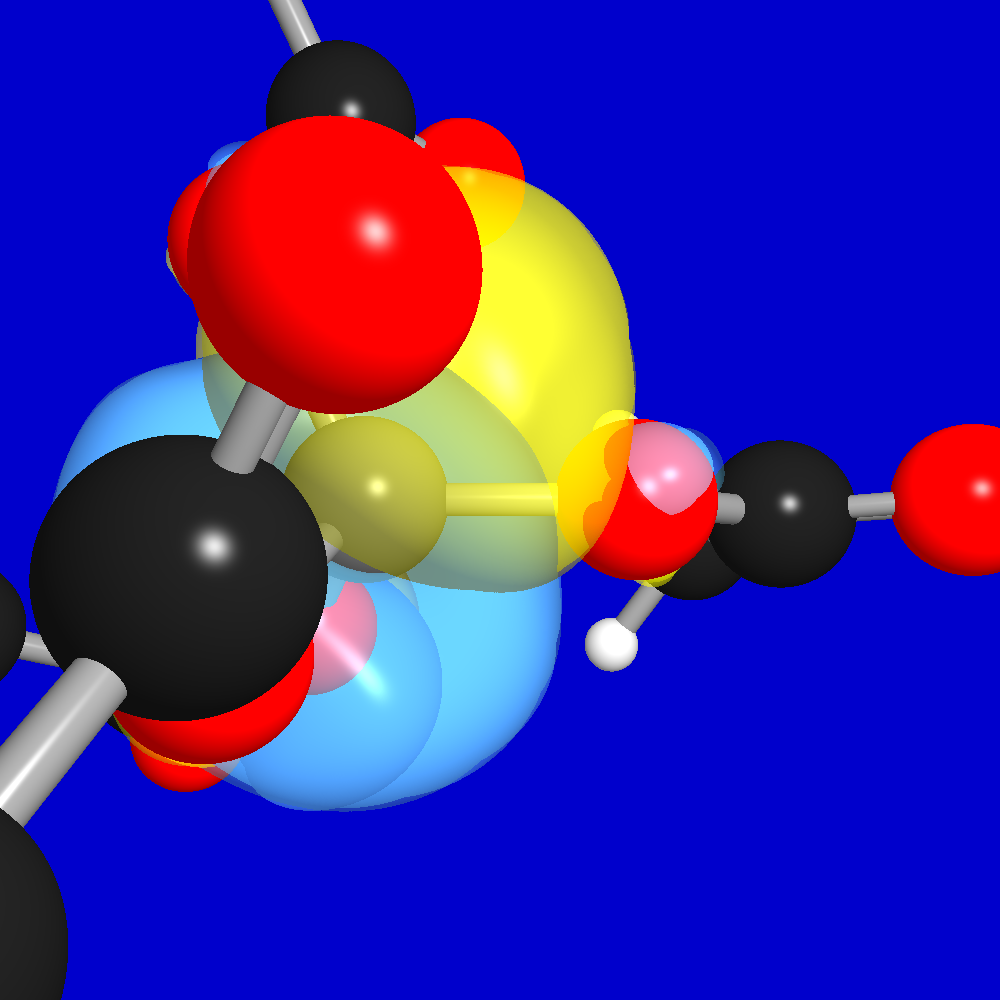
\includegraphics[width=6cm]{SI_AC_73.png}\label{}}
\label{prehled_nbo_SI_AC}
\end{center}
\end{figure}

\begin{figure}
\begin{center}
\caption{Přehled MPA \ce{Si(OAC)4};  Legedna: \mycircle{brown} Si, \mycircle{red} O, \mycircle{orange} C, \mycircle{yellow} P, \mycircleempty{black}~H}
\subfigure[MO 75 ]{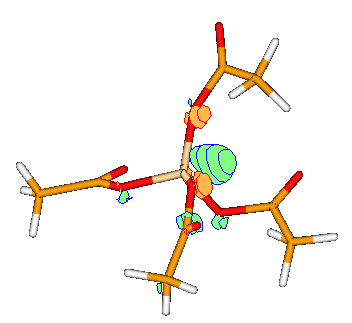
\includegraphics[width=6cm]{si_o_oac_4_75.png} \label{}}
\subfigure[MO 74]{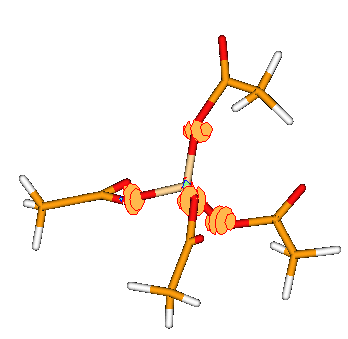
\includegraphics[width=6cm]{si_oac_74.png}\label{}}
\subfigure[MO 77]{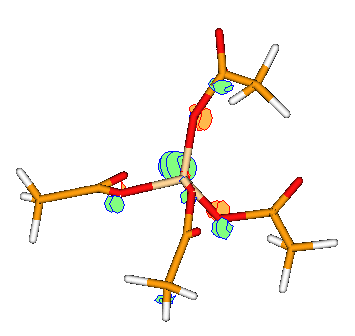
\includegraphics[width=6cm]{si_o_ac_4_77.png}\label{}}
\subfigure[MO 76]{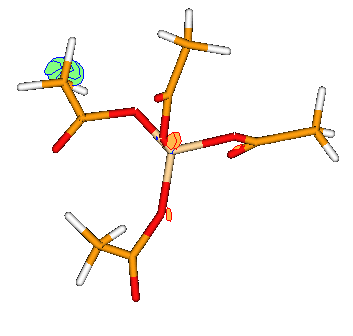
\includegraphics[width=6cm]{si_o_ac_4_76.png}\label{}}
\label{prehled_mpa_SI_AC}
\end{center}
\end{figure}

\begin{figure}
\begin{center}
\caption{Přehled MPA \ce{Si(CH3)(OAC)3};  Legedna: \mycircle{brown} Si, \mycircle{red} O, \mycircle{orange} C, \mycircle{yellow} P, \mycircleempty{black}~H}
\subfigure[MO 62 ]{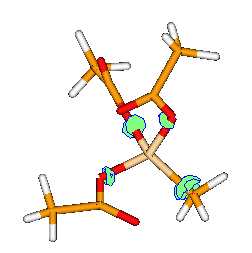
\includegraphics[width=6cm]{si_ch3_oac3_62.png} \label{}}
\subfigure[MO 63]{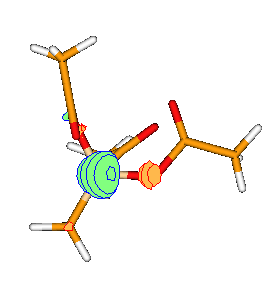
\includegraphics[width=6cm]{si_ch3_oac3_63.png}\label{}}
\subfigure[MO 64]{\includegraphics[width=6cm]{si_ch3_oac3_64.png}\label{}}
\subfigure[MO 65]{\includegraphics[width=6cm]{si_ch3_oac3_66.png}\label{}}
\label{prehled_mpa_SI_AC}
\end{center}
\end{figure}

\section{Spektroskopie}
 Poslední část, která se věnuje spektroskopii, dává pohled na NMR parametry křemíku a porovnává je s experimentálně získanými hodnotami. Experimentální hodnoty chemických posunů jsou uvedeny v \cite{1316862}. Hodnoty v tabulce \ref{nmr} jsou přepočítány na strandard, kterým byl tetramethyl silan s $\sigma_{TMS}$ 332,1 ppm.

\begin{table}[htbp]
\begin{minipage}{\textwidth}
\caption{Teoretické hodnoty NMR absolutního chemického stínění, $\sigma_{TMS}$ = 332,1 ppm,   \cite{1316862}.}
\begin{center}
\begin{tabular}{|l|l|r|l|r|r|r|}
\hline
\label{nmr} & \textbf{Q} & \textbf{R} &\textbf{S} & \textbf{P} & \textbf{O} & {exp \footnote{Experimentální hodnoty jsou ze článku \cite{1316862}} [ppm]} \\ \hline
central Si & -210,45 & -211,70 & -160,48 & -217,13 & -220,53 & -101 \\ \hline
4 Si & -161,26 & -157,15 &-158,26 & -164,78 & -161,25 & -212 \\ \hline
4. Si & -156,64 & -158,48 & -155,75 & -166,21 & -161,34 & -212 \\ \hline
4. Si & -159,50 & -157,32 &  & -164,28 & -163,01 & -212 \\ \hline
4 Si &  & -160,50 &  & -166,08 & -161,83 & -212 \\ \hline
4 Si &  & - &  & -168,73 & -161,46 & -212 \\ \hline
4 Si &  & - &  & -164,42 & -161,68 & -212 \\ \hline
\end{tabular}
\end{center}
\end{minipage}
\end{table}












\chapter{Závěr}
 Tato práce vznikla za podpory projektů CERIT Scientific Cloud (LM2015085) a~CESNET (LM2015042) financovaných z programu MŠMT Projekty velkých infrastruktur pro VaVaI.
\newpage
\chapter{Přílohy}
  \begin{lstlisting}[frame=single, caption={struktura koordinace 5},label=DescriptiveLabel]
OPT STRUKTURA_5_KOORDINACE

-1 1
Si      0.1060880     -0.1323080      1.0375270
O      1.5812970     -1.0976720      0.9967660
O      0.8974450      1.1240830      0.1688940
O     -1.4165630      0.7576620      0.9394990
O     -0.6552630     -1.3997120      0.0999750
O      0.0229970     -0.0776790      2.6855410
P      2.3564980     -2.3519490      0.4722700
P      2.2269690      1.9772360      0.2755320
P     -2.1096190      2.0277490      0.3627980
P     -2.1452450     -1.9360200      0.0266770
O      3.6707810     -1.7043880     -0.2463190
O      3.4776350      0.9812400      0.2257760
O     -3.6426970      1.5033340      0.2028160
O     -2.9965540     -0.9029920     -0.8705620
Si      4.0555520     -0.2021450     -0.7780110
Si     -4.2433870      0.1691170     -0.5698060
O      2.7547630     -3.3666980      1.4714960
O      2.3423360      2.4397160      1.8129550
O     -2.0097180      3.2994300      1.1181510
O     -2.8194110     -2.3356030      1.2840640
O      1.5297350     -2.9105480     -0.7944340
O      2.2723240      3.0744080     -0.7257780
O     -1.6921580      2.1504180     -1.1989060
O     -1.8688940     -3.1402730     -1.0193110
H      0.5973640     -2.6169910     -0.7313210
O      3.4719850     -0.0414510     -2.2987840
O      5.6860290     -0.0341030     -0.6943040
O     -4.8922530      0.5115670     -2.0304860
O     -5.4636920     -0.4526200      0.3064560
C      3.6740590      1.1071460     -3.1249710
H      3.2180050      0.8938780     -4.0964060
H      4.7447550      1.2999890     -3.2716820
H      3.2017280      1.9912910     -2.6852800
C      6.6006900     -1.1007480     -0.9118620
H      7.5927530     -0.7573280     -0.6016910
H      6.6426240     -1.3786210     -1.9736040
H      6.3274260     -1.9850090     -0.3259560
C     -0.9849770      3.3107900     -1.6773210
H      0.0860700      3.2086990     -1.4896040
H     -1.3635080      4.2155590     -1.1940220
H     -1.1729450      3.3571590     -2.7538780
C     -2.9263860     -4.0733420     -1.2662770
H     -2.4914580     -4.8847540     -1.8535360
H     -3.7322580     -3.5983060     -1.8380380
H     -3.3245040     -4.4647010     -0.3252780
C     -4.1337720      0.8029070     -3.1996090
H     -3.6537510      1.7841190     -3.1197100
H     -4.8254030      0.8072490     -4.0481970
H     -3.3592180      0.0467850     -3.3704670
C      1.4798560      3.5121350      2.2509330
C      0.9413100     -0.6499850      3.6071830
H      0.4787970     -0.5857820      4.5985100
H      1.8840520     -0.0904060      3.6163660
H      1.1623230     -1.6960460      3.3772890
H      0.4247060      3.2699000      2.0910820
H      1.7314910      4.4345160      1.7187700
H      1.6728370      3.6308940      3.3186740
C     -5.4960610     -0.5265130      1.7357500
H     -6.5126110     -0.8157020      2.0201440
H     -5.2624300      0.4468630      2.1811820
H     -4.7807210     -1.2730840      2.0905780

  \end{lstlisting}


\newpage

  \begin{lstlisting}[frame=single, caption={puvodni struktura C cis} ,label=DescriptiveLabel]
OPT STRUKTURA_C_CIS

0 1
Si      0.4362750     -0.3308130      0.1798660
O      0.0302110      1.4468910      0.7261310
O     -0.8564990     -0.0851840     -0.9735320
O      1.7846080     -0.3744530      1.2821930
O     -0.6146920     -1.0436500      1.3726750
O      1.6144150      0.6336900     -0.9892260
O      0.8847720     -1.7877540     -0.6288930
C     -0.3438780      2.0694820      1.7462750
C      2.1261230      0.4547880     -2.1168400
C      1.4460740     -0.1836080     -3.2746040
C      0.1437130      1.8089160      3.1263220
H      0.1330580      0.7345630      3.3131440
H     -0.4661440      2.3412640      3.8549450
H      1.1944900      2.1250230      3.1698980
O     -1.1423970      3.0922300      1.5849480
O      3.3558730      0.8717880     -2.3015790
P     -1.8581550      0.8733550     -1.6896390
P     -2.1537160     -0.8810520      1.7000150
P      1.1394150     -3.3042950     -0.3141620
P      3.1847420      0.2572400      1.6064990
O     -2.3569670      1.9699320     -0.6241930
O     -3.1768000     -0.0354590     -1.8132940
O     -1.4188810      1.4575590     -2.9784610
O      3.9974000     -0.8958370      2.3558520
O      4.0607640      0.3011950      0.2398030
O      3.1507920      1.5794480      2.2877420
O      1.8693300     -3.6936310     -1.7037000
O      1.8625800     -3.6820430      0.9259450
O     -2.9628540     -1.5079350      0.4757860
O     -2.5522520      0.4936190      2.1082600
Si     -3.9291290     -1.1344810     -0.8109850
Si      4.3329560      1.3821040     -0.9707700
Si     -2.0676360      3.3779690      0.1680340
O     -5.3261160     -0.5300350     -0.2355970
O     -4.2248350     -2.4817130     -1.6730560
O     -1.2080000      4.4596480     -0.6715700
O     -3.4830900      3.9756990      0.6855210
O      3.9269550      2.9239010     -0.7340590
O      5.8713020      1.2271510     -1.4640700
C     -3.2757870     -3.1504890     -2.5107140
C     -6.4428220     -0.1892290     -1.0585370
C     -1.4548990      4.8532830     -2.0302510
C     -4.5039280      3.2083100      1.3424620
C      4.4478990      3.8109950      0.2696730
C      6.6504170      0.0279030     -1.4497830
H      6.3830590     -0.6085400     -2.3006320
H      6.5030490     -0.5281290     -0.5186480
H      5.5347860      3.9038070      0.1704730
H      4.1833280      3.4413070      1.2631890
H      2.0814950     -0.1423500     -4.1590900
H      0.4893380      0.3250900     -3.4470630
H     -5.3332800      3.8893260      1.5471930
H     -4.1289850      2.7853660      2.2785850
H     -1.4666020      3.9799650     -2.6893850
H     -0.6411420      5.5208710     -2.3220650
H     -6.7922250     -1.0600210     -1.6237990
H     -6.1841610      0.6157000     -1.7565350
H     -2.3855900     -3.4446420     -1.9447500
H     -2.9787990     -2.5067960     -3.3462170
H      1.2280720     -1.2231410     -3.0064460
O     -2.4310020     -2.0397870      2.7810730
O     -0.2884920     -4.0561990     -0.4702960
C     -1.8387150     -1.9197020      4.0848920
H     -2.2601130     -2.7259420      4.6873340
H     -2.0902250     -0.9542090      4.5348850
H     -0.7521140     -2.0363440      4.0198160
C     -0.9103980     -4.6776960      0.6731820
H     -1.5848650     -5.4399090      0.2767870
H     -1.4827170     -3.9400780      1.2399400
H     -0.1566580     -5.1371200      1.3167040
C      3.3434860     -1.8341050      3.2376550
H      4.1487010     -2.4078190      3.7000480
H      2.6905660     -2.4915460      2.6602710
H      2.7851710     -1.3076660      4.0196210
C      2.3129820     -5.0478520     -1.8712030
H      2.8722290     -5.0766000     -2.8083250
H      1.4555660     -5.7266400     -1.9352560
H      2.9615330     -5.3473950     -1.0422170
H     -7.2437530      0.1541510     -0.3989960
H     -4.8454950      2.3891910      0.7023420
H      3.9887110      4.7870780      0.0988820
H      7.6999750      0.3183380     -1.5382370
H     -3.7652420     -4.0447310     -2.9050930
H     -2.4044580      5.3944290     -2.1044270

  \end{lstlisting}
 \newpage
  \begin{lstlisting}[frame=single, caption={puvodni struktura C trans },label=DescriptiveLabel]
OPT STRUKTURA_C_TRANS

0 1
Si      0.1568620      0.0982880     -0.4546840
O     -1.3858890     -0.0173790     -1.2768970
O     -0.3952950     -1.3151690      0.6399790
O      1.6543810      0.2513780      0.4670240
O      0.5816890      1.4511660     -1.6650310
O     -0.5550920      1.2242170      0.7165680
O      0.8678080     -1.0493540     -1.5450430
P     -2.7196520     -0.8175830     -1.3999680
P     -1.5614130      2.4311220      0.6006710
P      1.5991580     -2.4289430     -1.5513710
P      3.1575710      0.5538690      0.1400790
C     -0.4911750     -1.8030960      1.7766270
C      1.1168160      2.5701510     -1.5429810
O     -2.8614740     -1.8238840     -2.4689240
O      2.4652110     -2.7355600     -2.7095090
O      3.5246940      0.7921840     -1.2810010
O     -1.3775150      3.3864190     -0.5206460
O     -3.0523280     -1.4172600      0.0875580
O     -3.8310160      0.3473290     -1.4758010
O     -3.0346810      1.7728760      0.6776300
Si     -4.2709810      1.5404840     -0.4030280
O     -5.5155180      1.0761000      0.5493300
O     -4.7174780      2.8446060     -1.2603230
C     -6.8440280      0.8962360      0.0549760
H     -7.4810840      0.6455980      0.9072710
H     -6.8847240      0.0775730     -0.6733780
C     -4.0819080      3.3580460     -2.4379070
H     -3.9519420      2.5655430     -3.1827420
H     -3.1099430      3.7855500     -2.1798310
Si     -2.8613170     -2.7890720      0.9651670
O     -1.5276080     -2.5541570      2.0522850
O     -4.1505110     -2.9825080      1.9321820
C     -4.8705630     -1.9516350      2.6152870
H     -5.0445180     -1.0866570      1.9676180
H     -4.3193470     -1.6345360      3.5082770
O      2.3989500     -2.5130800     -0.1252060
O      3.9863780     -0.5947040      0.8758450
Si      3.8841800     -2.2433030      0.5209140
O      3.4932430      1.8594190      1.0534360
Si      2.9221630      3.3281230      0.5346430
O      1.5450890      3.0122770     -0.3922010
O      3.9902590      4.1448810     -0.3736060
O      5.1609740     -2.6986570     -0.3649740
O      3.8702300     -3.0512760      1.9399110
C      5.2331590      3.6780950     -0.9225550
H      5.5411230      4.4027560     -1.6799600
H      5.1110330      2.6919880     -1.3776890
C      5.5585970     -2.1731050     -1.6455000
H      5.6199210     -1.0806660     -1.6126190
H      4.8353460     -2.4710640     -2.4081360
C      4.9833830     -3.0947720      2.8342050
H      5.8673780     -3.5100060      2.3386400
H      4.7075330     -3.7397940      3.6724430
C      0.5272200     -1.6233640      2.8512710
H      0.9053030     -0.5994870      2.8206430
H      1.3742560     -2.2866450      2.6315300
H      0.1134810     -1.8768470      3.8277250
C      1.2031660      3.4833650     -2.7173080
H      2.1513140      4.0263560     -2.7029680
H      0.3858230      4.2068130     -2.6083180
H      1.0760720      2.9258250     -3.6451230
O      2.3967930      4.1564720      1.8176540
O     -1.4421630      3.1733550      2.0212940
O     -2.5037560     -4.1488260      0.1746090
O      0.4004360     -3.4653990     -1.2702190
C     -3.2605790     -4.7033860     -0.9189600
C      0.6784730     -4.8715240     -1.3640650
H      1.4342270     -5.1659420     -0.6269970
H      1.0237220     -5.1272260     -2.3693510
H     -0.2608670     -5.3783540     -1.1418880
C     -1.6169880      2.4590950      3.2520580
H     -1.5203120      3.1958520      4.0515040
H     -2.6102140      2.0008760      3.2924490
H     -0.8435050      1.6929060      3.3629410
C      1.4930470      5.2697650      1.7928560
H      0.5621890      5.0014240      1.2850080
H      1.9575300      6.1315050      1.3009770
H     -2.7733910     -5.6399930     -1.1986650
H     -3.2562860     -4.0117130     -1.7647800
H      5.2181540     -2.0938720      3.2155740
H      6.5435780     -2.5906160     -1.8677800
H     -5.8291390     -2.3749400      2.9255210
H      1.2739670      5.5282440      2.8309780
H      5.9955110      3.6342350     -0.1381040
H     -7.2153150      1.8141500     -0.4127620
H     -4.2864410     -4.9188870     -0.6010600
H     -4.7363320      4.1328280     -2.8456680

  \end{lstlisting}


{\csname captions\languagename\endcsname %% Temporarily override
%% the BibLaTeX localization with the original babel definitions.
\makeatletter %% Use the correct localization of the quotations.
  \thesis@selectLocale{\thesis@locale}\makeatother
\printbibliography[heading=bibintoc]} %% Print the bibliography.
\appendix %% Start the appendices.




\end{document}
